
Following the discussion of neutrino physics and the significance of neutrinoless double beta decay, this chapter introduces the LEGEND experiment, a next-generation effort to search for neutrinoless double beta decay. It builds on the advancements of its predecessors, MJD and GERDA. LEGEND reuses the infrastructure at the Laboratori Nazionali del Gran Sasso (LNGS), previously used by GERDA, and upgrades it to improve both background suppression and detector performance. 
The chapter begins with a short overview of how LEGEND evolved from GERDA and MAJORANA, focusing on key improvements in detector design and instrumentation. It then introduces the high-purity germanium (HPGe) detectors used in the experiment, and the principles of semiconductor physics, including doping and charge collection. Finally, it covers how these detectors are used to identify neutrinoless double beta decay events, how pulse shape discrimination (PSD) helps to reject background, and how the detectors are calibrated in LEGEND-200. 

\subsection{From GERDA to LEGEND}

The GERmanium Detector Array (GERDA) aimed to search for $0 \nu \beta \beta$ decays using high-purity germanium detectors enriched to 87\% in $^{76}$Ge. Located at LNGS, the setup was shielded by 3500 meters of water equivalent of rock, significantly reducing the cosmogenic background.
GERDA operated in two phases. Phase I reached a background index of $10^{-2}$~counts/(keV$\cdot$kg$\cdot$yr) with a total exposure of $21.6 \; \mathrm{kg} \cdot \mathrm{yr}$. The experiment set a new lower limit on the half-life of $T^{0 \nu}_{1/2} > 2.1 \times 10^{25}$yr (90\% CL). 
In phase II, the goal was to improve sensitivity by an order of magnitude. This was addressed by introducing a new detector geometry with better energy resolution and improved pulse shape discrimination (BEGe detectors), as well as a new liquid argon (LAr) veto system and a denser detector array~\cite{agostini_upgrade_2018}. 

In GERDA, the HPGe detectors were attached on strings and submerged in a cryostat filled with 64 m$^3$ LAr, which served both as a coolant and as an active shield against background radiation, including cosmic and environmental radiation. Surrounding the cryostat was a 590 m$^3$ ultra-pure water tank equipped with 66 PMTs providing Cherenkov veto against muons. The clean room was located above the cryostat~\cite{agostini_upgrade_2018}. 
Within the LAr volume, an additional veto system detected energy deposits in both the germanium detectors and the LAr, with scintillation light being measured through wavelength-shifting fibers. These fibers converted the 128 nm scintillation light into green light, directing the photons to silicon photomultipliers for precise detection~\cite{agostini_upgrade_2018}.  

The LEGEND experiment continues from both GERDA and MJD. The idea is to combine GERDA's low background techniques with the high energy resolution of MJD. The final stage, LEGEND-1000, is planned to consist of 1000 kg of germanium and aims for a discovery sensitivity on the order of $10^{28}$ years at $99.7$\% C.L.~\cite{abgrall_large_2017}. 
In a first step, LEGEND-200 aims to employ 200 kg of HPGe detectors inside the existing infrastructure of GERDA, combining it with the low-noise electronics of the MAJORANA experiment, which was achieved by using low-mass front-end electronics close to the detector. The goal is to enter the background-free regime, which is defined as having $< 1$ expected background counts in the region of interest over the experiment's exposure~\cite{collaboration_legend-1000_2021}. For LEGEND-200, this corresponds to a background index of $2 \times 10^{-4} \mathrm{counts / (keV \cdot kg \cdot yr)}$. The design of the LEGEND-200 detector setup is shown in figure~\ref{fig:l200_design}. 

\begin{figure}
    \centering
    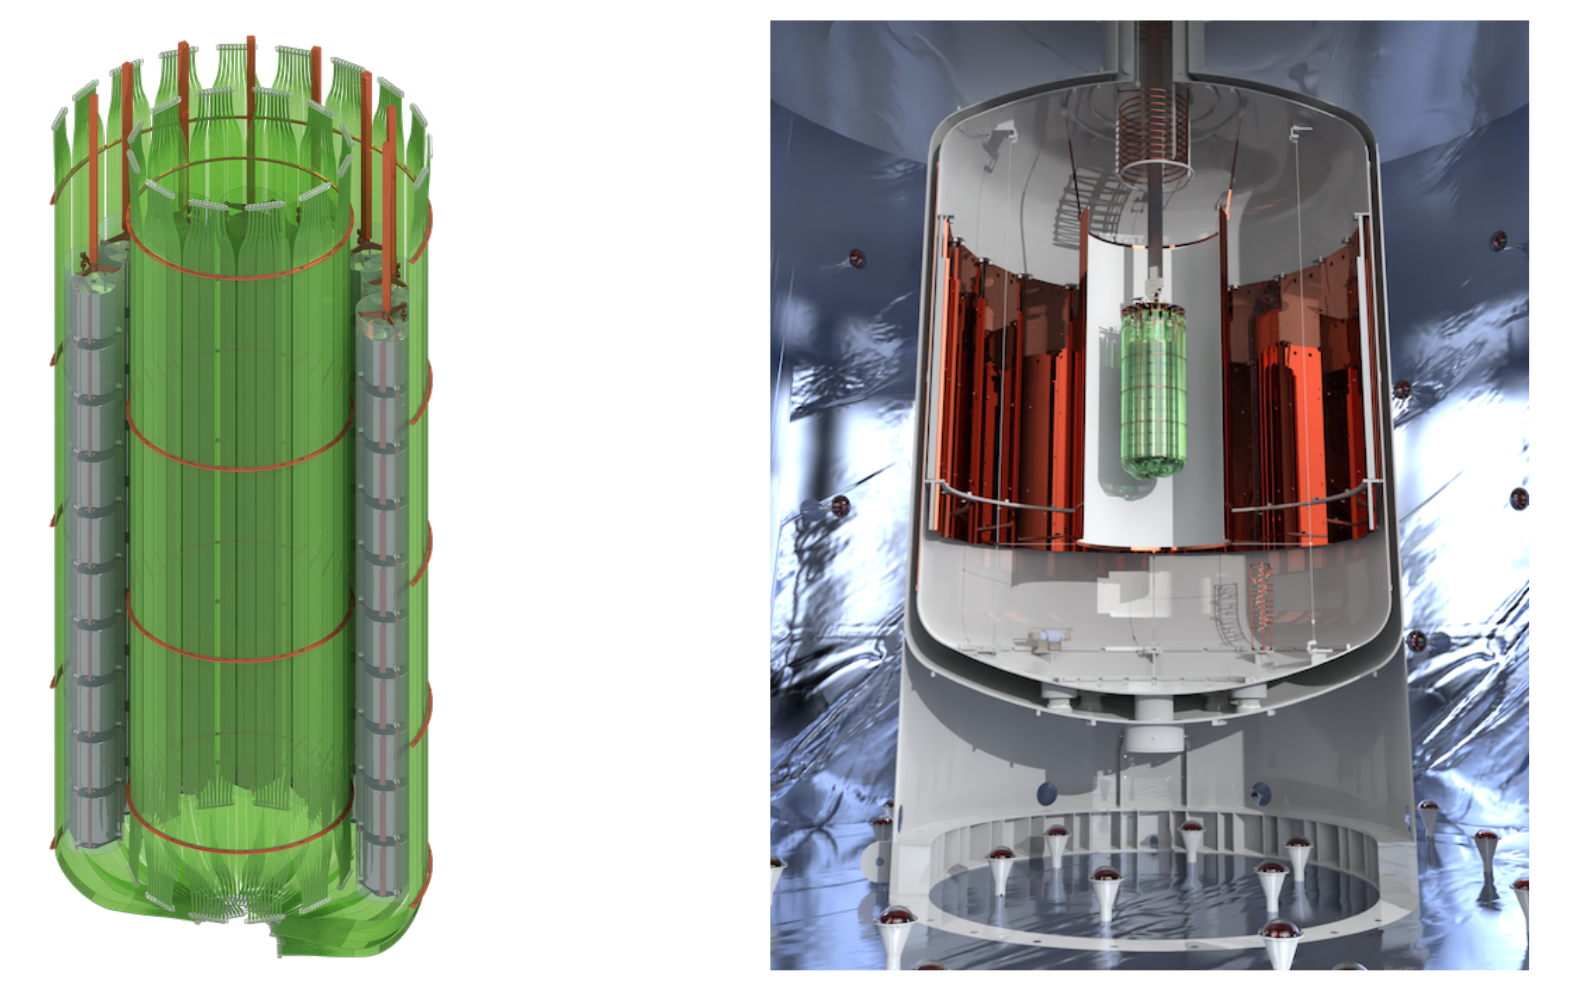
\includegraphics[width=0.8\linewidth]{figures/03_legend/LEGEND_200_design.png}
    \caption{LEGEND-200 design. The left image shows the germanium detectors mounted on the strings, surrounded by optical fibers that guide the LAr scintillation light to silicon photomultipliers. 
	The right image shows the cryostat located in the water Cherenkov tank, which is equipped with PMTs to detect coincident muons~\cite{collaboration_legend-1000_2021}.}
    \label{fig:l200_design}
\end{figure}


\subsection{Germanium detectors}
High-purity germanium detectors are at the core of the LEGEND experiment. Their excellent energy resolution and ability to reconstruct interaction topologies make them particularly well suited for $0 \nu \beta \beta$ decay searches. 

\subsubsection{Germanium semiconductors}
In crystalline solids like germanium, the periodic atomic structure gives rise to a quasi-continuum of energy levels known as energy bands. The valence band is the highest band fully occupied by electrons, while the conduction band is the lowest unoccupied band. The energy difference between these two bands is called the band gap, and its value determines the material's electrical properties. In conductors, the bands overlap; in insulators, the band gap is large. Semiconductors fall in between with band gaps typically below $<3$~eV.  
In the case of germanium, the band gap is $0.67$~eV~\cite{hofmann_solid_2015}. Each atom contributes four electrons that form covalent bonds with neighboring atoms. At zero temperature, the valence band is completely filled and the conduction band is empty, resulting in a very low electrical conductivity. 
However, at non-zero temperatures, thermal excitation can promote electrons into the conduction band, creating electron-hole pairs. Holes represent the absence of electrons in the valence band and act as positively charged carriers. Although the ions themselves are stationary, the movement of holes contributes to electrical conduction~\cite{hofmann_solid_2015, simon_oxford_2017}. 
The law of mass action relates the concentration of electrons $n$ and holes $h$ in a semiconductor at thermal equilibrium: 

\begin{equation}
\label{eq:law_of_mass_action}
	n \cdot p = \text{constant} \,.
\end{equation}

For a perfectly pure semiconductor at room temperature, the charge carrier concentrations are very low, resulting in correspondingly low electrical conductivity. However, in practice, there are always small amounts of impurities present, which increase the number of free charge carriers and thereby the conductivity. 
There are two important types of electronically active impurities: Atoms that act as electron donors are called n-type, while atoms that readily accept electrons (and thus effectively donate holes) are referred to as p-type. 
Semiconductors are typically doped with either type to increase the conductivity to a reasonable value. 
For tetravalent elements like germanium, n-type doping is achieved by introducing pentavalent atoms like phosphorus. The additional outer shell electron cannot participate in a covalent bond and remains only loosely bound to the positively charged nucleus. Its energy level lies just below the conduction band, and only a small amount of thermal energy is required to excite it into the conduction band ~\cite{sze_semiconductor_2012, hofmann_solid_2015, knoll_radiation_2000}. 
P-type doping is achieved by adding trivalent atoms such as boron or aluminium, which act as electron acceptors with energy levels just above the valence band.
At high enough temperatures, where the electrons are no longer bound to the dopant atoms, n-type doping will lead to free electrons and p-type doping leads to free holes, thus increasing the free charge carrier concentration in either case. Regions with very high doping concentrations are particularly well suited for electrical contacts due to their high conductivity. These regions are referred to $n^{+}$ and $p^{+}$, depending on the type of impurity introduced~\cite{simon_oxford_2017, knoll_radiation_2000}. 


\subsubsection{Semiconductors as particle detectors}
If p-type and n-type semiconductors are brought into direct contact, the concentration gradient causes electrons to diffuse into the p-doped region, while holes diffuse towards the n-doped region. In the overlapping region, known as the depletion zone, electrons and holes recombine. For each electron that diffuses away from the n-doped side, a net positive charge remains due to the immobile donor impurity. 
Analogously, for every hole that diffuses out of the p-doped side, an immobile acceptor impurity remains. This charge imbalance creates an electric field across the depletion region, which acts to counter further diffusion until equilibrium is reached~\cite{knoll_radiation_2000, simon_oxford_2017}. 
The depletion region contains almost no free charge carriers and therefore exhibits very high resistivity. 


\begin{figure}[t]
    \centering
    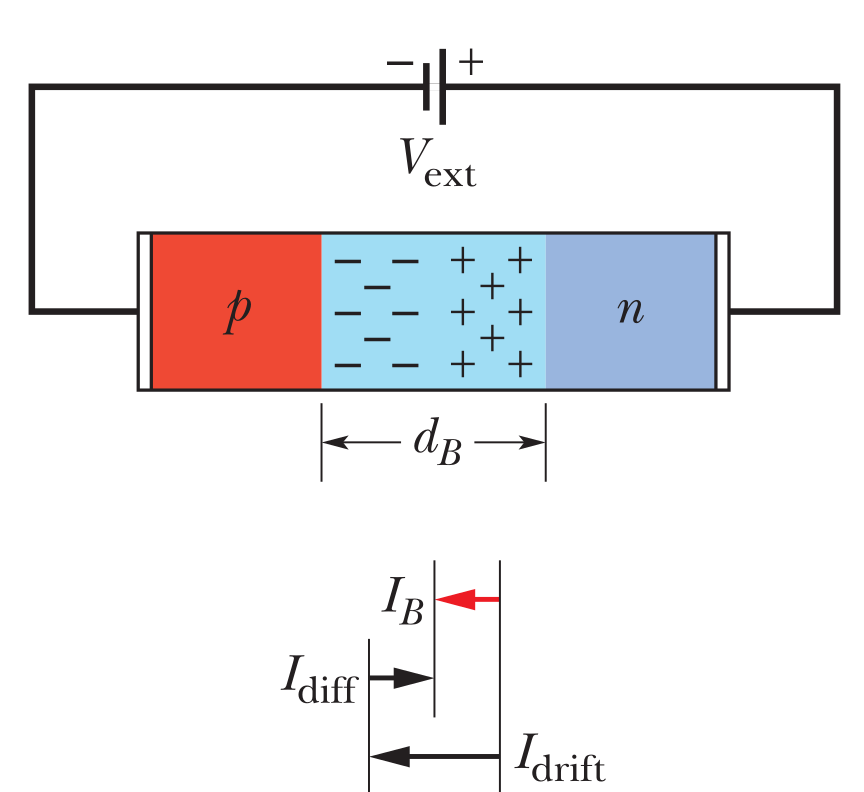
\includegraphics[width=0.5\linewidth]{figures/03_legend/PN_junction.png}
    \caption{Schematic view of a p-n junction in reverse bias. Since the applied voltage opposes the direction of the diffusion $I_{\text{diff}}$, only a small current $I_B$ remains. As a result, the depletion zone $d_B$ widens and the conductivity decreases~\cite{walker_fundamentals_2014}.}
\label{fig:pn_junction}
\end{figure}

 
An external voltage can be applied across the junction in either direction: 
When the voltage is applied in the same direction as the concentration difference (i.e., opposite the existing electric field), the junction is said to be in forward bias. In this case, electrons can move easily from the n-doped to the p-doped region, and the conductivity increases. 

The reverse case is more relevant for particle detection. In reverse bias, which is shown in figure~\ref{fig:pn_junction}, the external voltage is applied in the same direction as the existing electric field, opposing the natural diffusion of charge carriers. This pulls electrons from the p-doped region toward the n-side. Since the carrier concentrations are already low, the current is greatly suppressed, and the depletion region widens ~\cite{hofmann_solid_2015, knoll_radiation_2000, simon_oxford_2017}.

When ionizing radiation interacts in the depletion zone of a reverse-bias semiconductor, it deposits energy and generates a number of electron-hole pairs within a few picoseconds~\cite{agostini_pulse_2022}. 
These charge carriers are separated by the electric field and drift towards their respective electrodes, inducing a measurable signal. Due to the low ionization energy in semiconductors, detectors of this type achieve a high signal-to-noise ratio. 
The probability for such interactions, and its dependence on photon energy in germanium, is illustrated in figure~\ref{fig:Ge_attenuation}, which shows the mass attenuation coefficient for germanium, including prominent K- and L-shell absorption edges. 

\begin{figure}
    \centering
    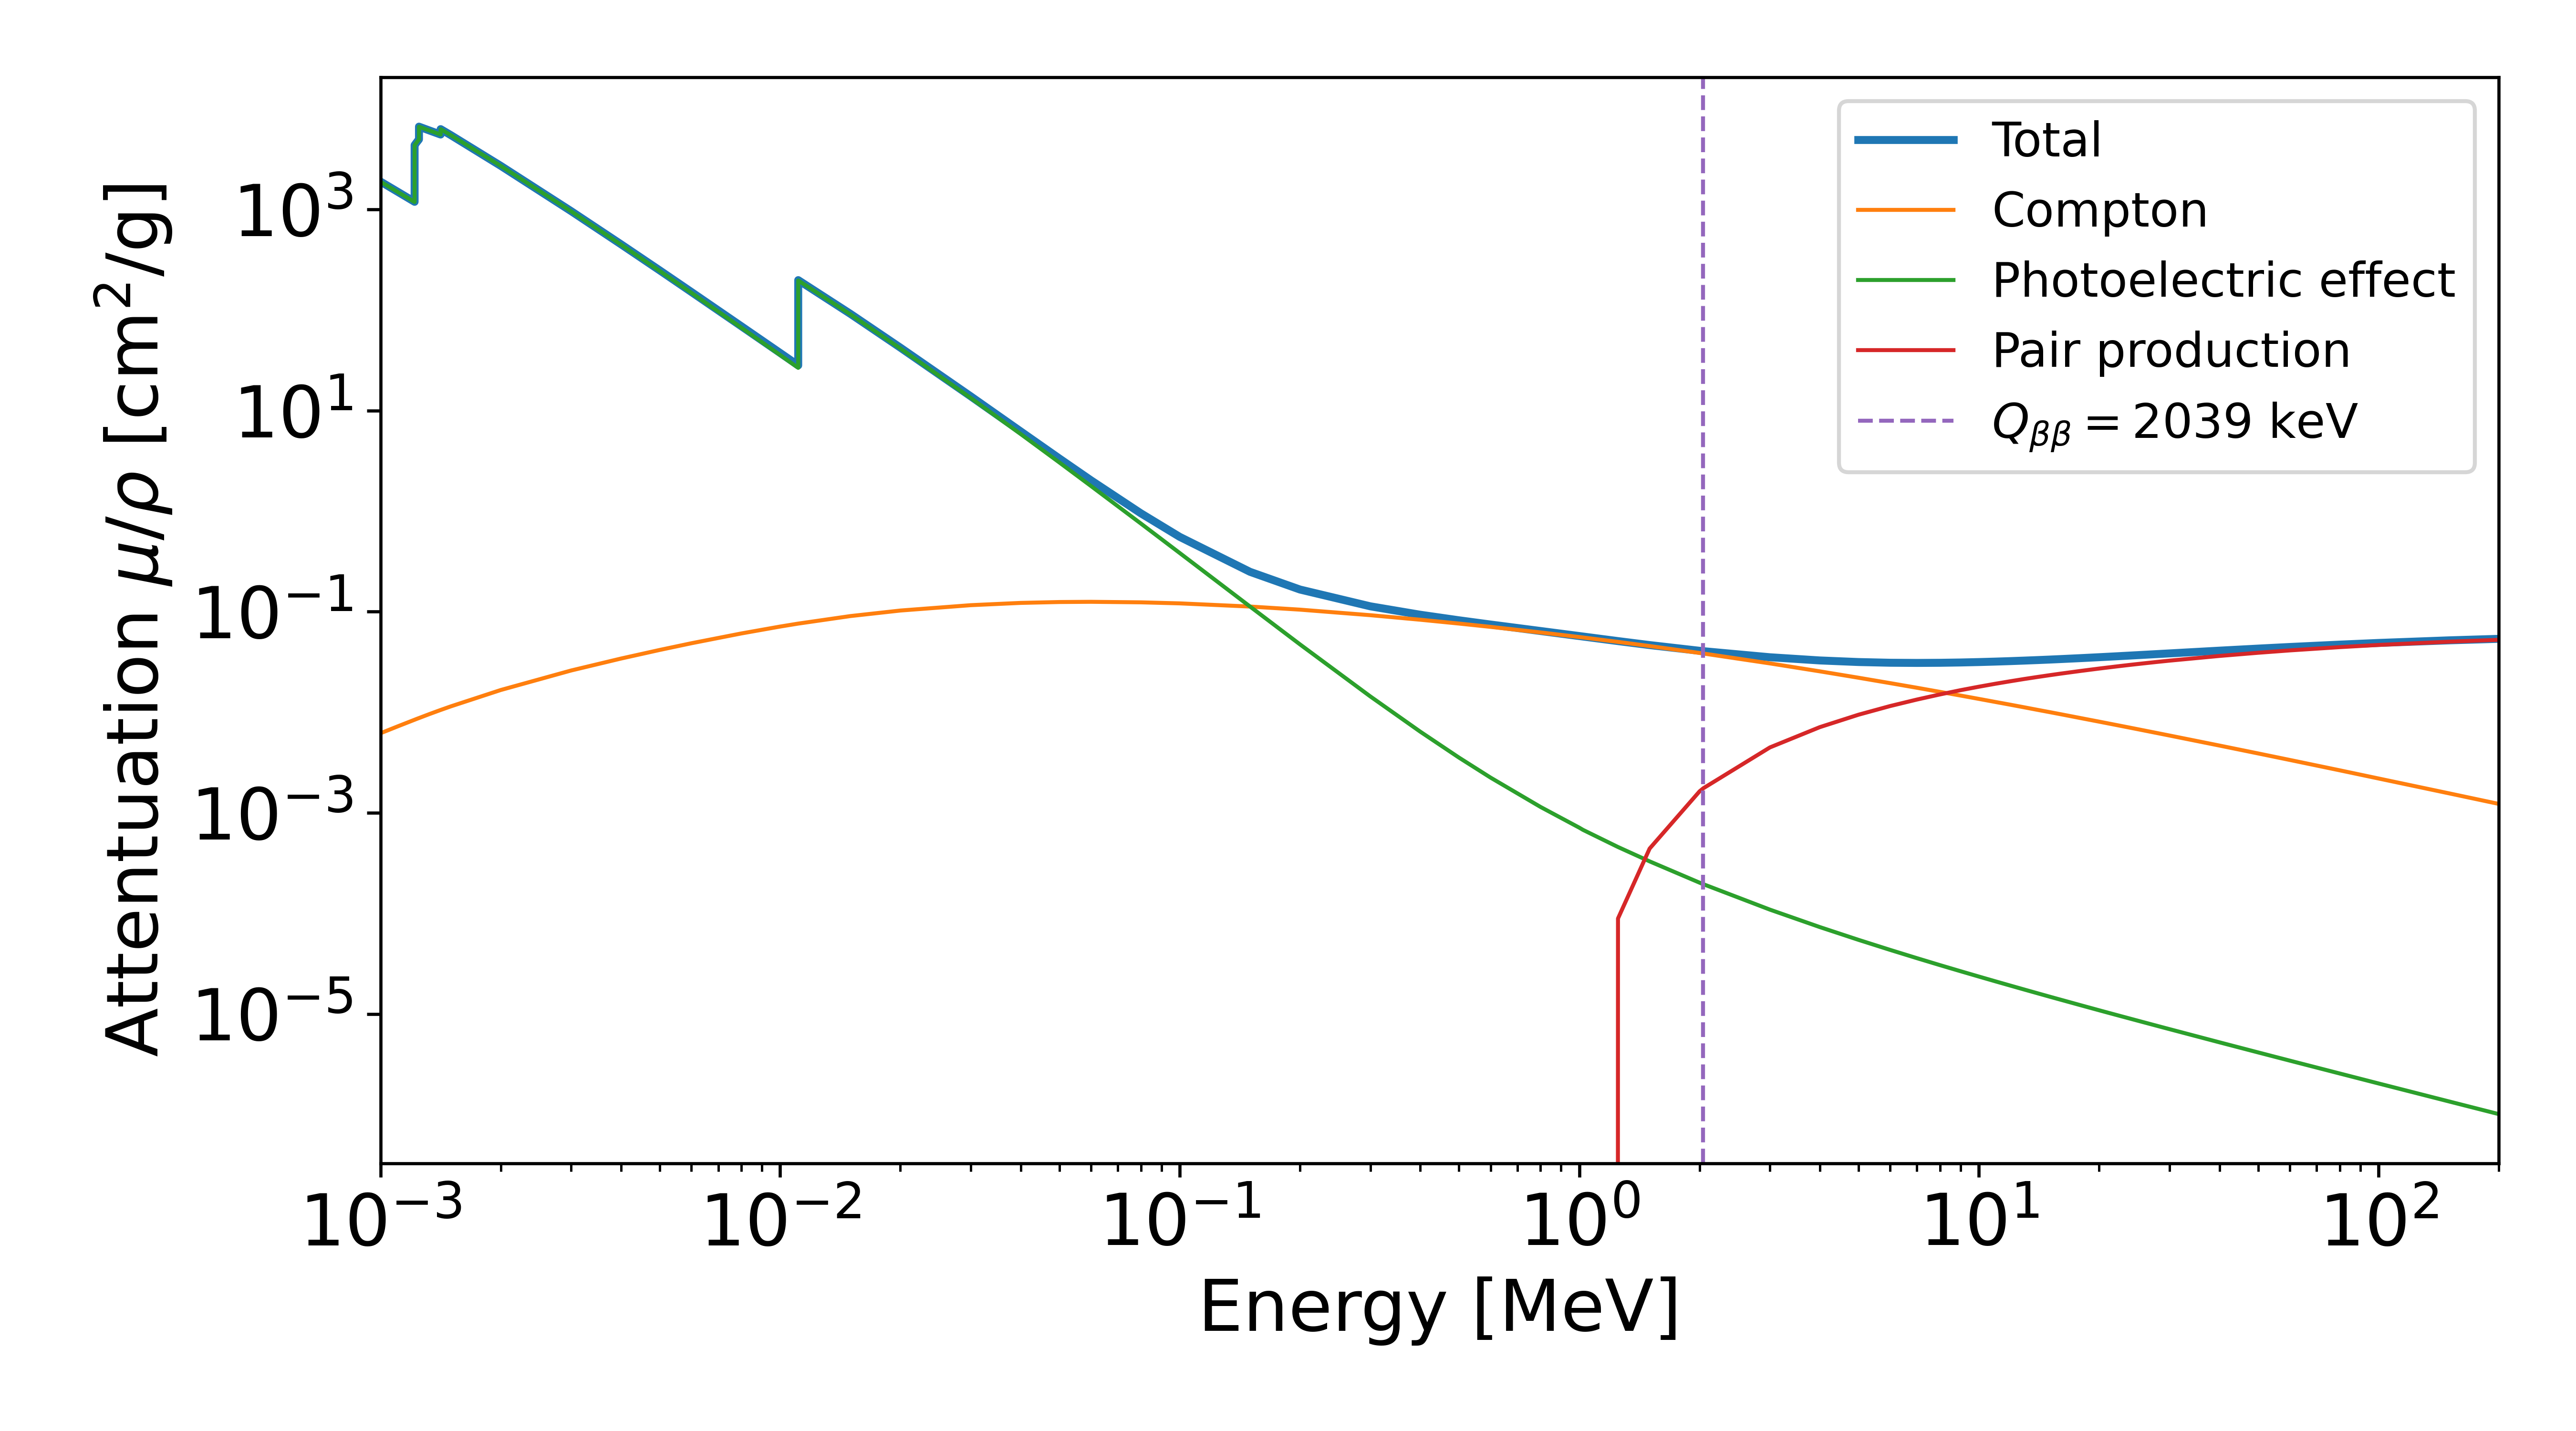
\includegraphics[width=0.75\linewidth]{figures/03_legend/Attentuation_germanium.png}
    \caption{Mass attenuation coefficients for germanium, showing contributions from photoelectric absorption, incoherent (Compton) scattering, and pair production, along with the total attenuation. The region of interest around $Q_{\beta \beta}$ (horizontal line) is dominated by Compton scattering. Data from NIST XCOM~\cite{nist_xcom_1999}.}
\label{fig:Ge_attenuation}
\end{figure}

In HPGe detectors, the applied reverse bias is large enough to deplete almost the entire detector volume, but still below the breakdown voltage. The small region that remains undepleted is referred to as dead layer, where charge collection is incomplete and signals are suppressed~\cite{knoll_radiation_2000}. 

The electron-hole pairs created during an interaction inside the detector drift toward the electrodes in a few microseconds. 
While in principle signals can be read out from either p$^+$ or n$^+$ electrode of the detector, the point-contact detectors in LEGEND-200 always read from the p$^{+}$ electrode. 
In LEGEND-200, the HPGe diodes are operated at 77~K, where the typical charge carrier drift velocities are on the order of $10^{7}$~cm/s~\cite{comellato_charge_2021}. 

The measured signal does not result from the collection of discrete charges at the electrode itself, but rather from the movement of the charge carriers, which induces a current in the electrodes. 
The induced charge can be determined by integrating the normal component of the electric field $\vec{E}$ over the surface $\vec{S}$ surrounding the electrode: 

\begin{equation}
\label{eq:Q_ind_original}
	Q = \oint_S \epsilon \vec{E} \cdot d \vec{S} \,,
\end{equation}

\noindent where $\epsilon$ is the dielectric constant of the material. To achieve precise charge reconstruction, the electric field must, in principle, be calculated for many points along the carriers' trajectories~\cite{he_review_2001}. 
However, this can be simplified using the Ramo-Shockley theorem~\cite{ramo_currents_1939, shockley_currents_1938}, which allows for the induced charge to be calculated more efficiently. In this approach, the readout electrode is set to 1 volt while all other electrodes are grounded. The induced charge from a single moving charge $q$ at position $x(t)$ is then: 

\begin{equation}
\label{eq:Shockley_ramo_theorem}
	Q_{ind}(x(t)) = -q \cdot \varphi_0{(x(t))} \,.
\end{equation}

The electric potential $\varphi_0$ is the weighting potential, and it only needs to be computed once for a given geometry. 
In most applications, it is assumed that all charge carriers are created at a single position in the active volume and that the electric field is strong enough for the charge carriers to reach saturated drift velocity. 
The total induced charge includes contributions from both electron and hole movement. For a planar detector geometry with thickness $d$, the induced charge can be expressed as

\begin{equation}
\label{}
	Q_{ind} = \frac{q_0}{d} \left( \text{electron drift distance} + \text{hole drift distance} \right) \,,
\end{equation}

\noindent where $q_0$ determines the maximum induced charge. It is defined as $q_0 =  N \cdot e$ with $N$ being the number of electron-hole pairs and $e$ the electronic charge. 
Depending on the location of the energy deposition, either electrons or holes may dominate the signal. This results in characteristic pulse shapes, as illustrated in figure~\ref{fig:Pulse_shape}. The general concept also applies to more complex detector geometries~\cite{knoll_radiation_2000}.  

\begin{figure}
    \centering
    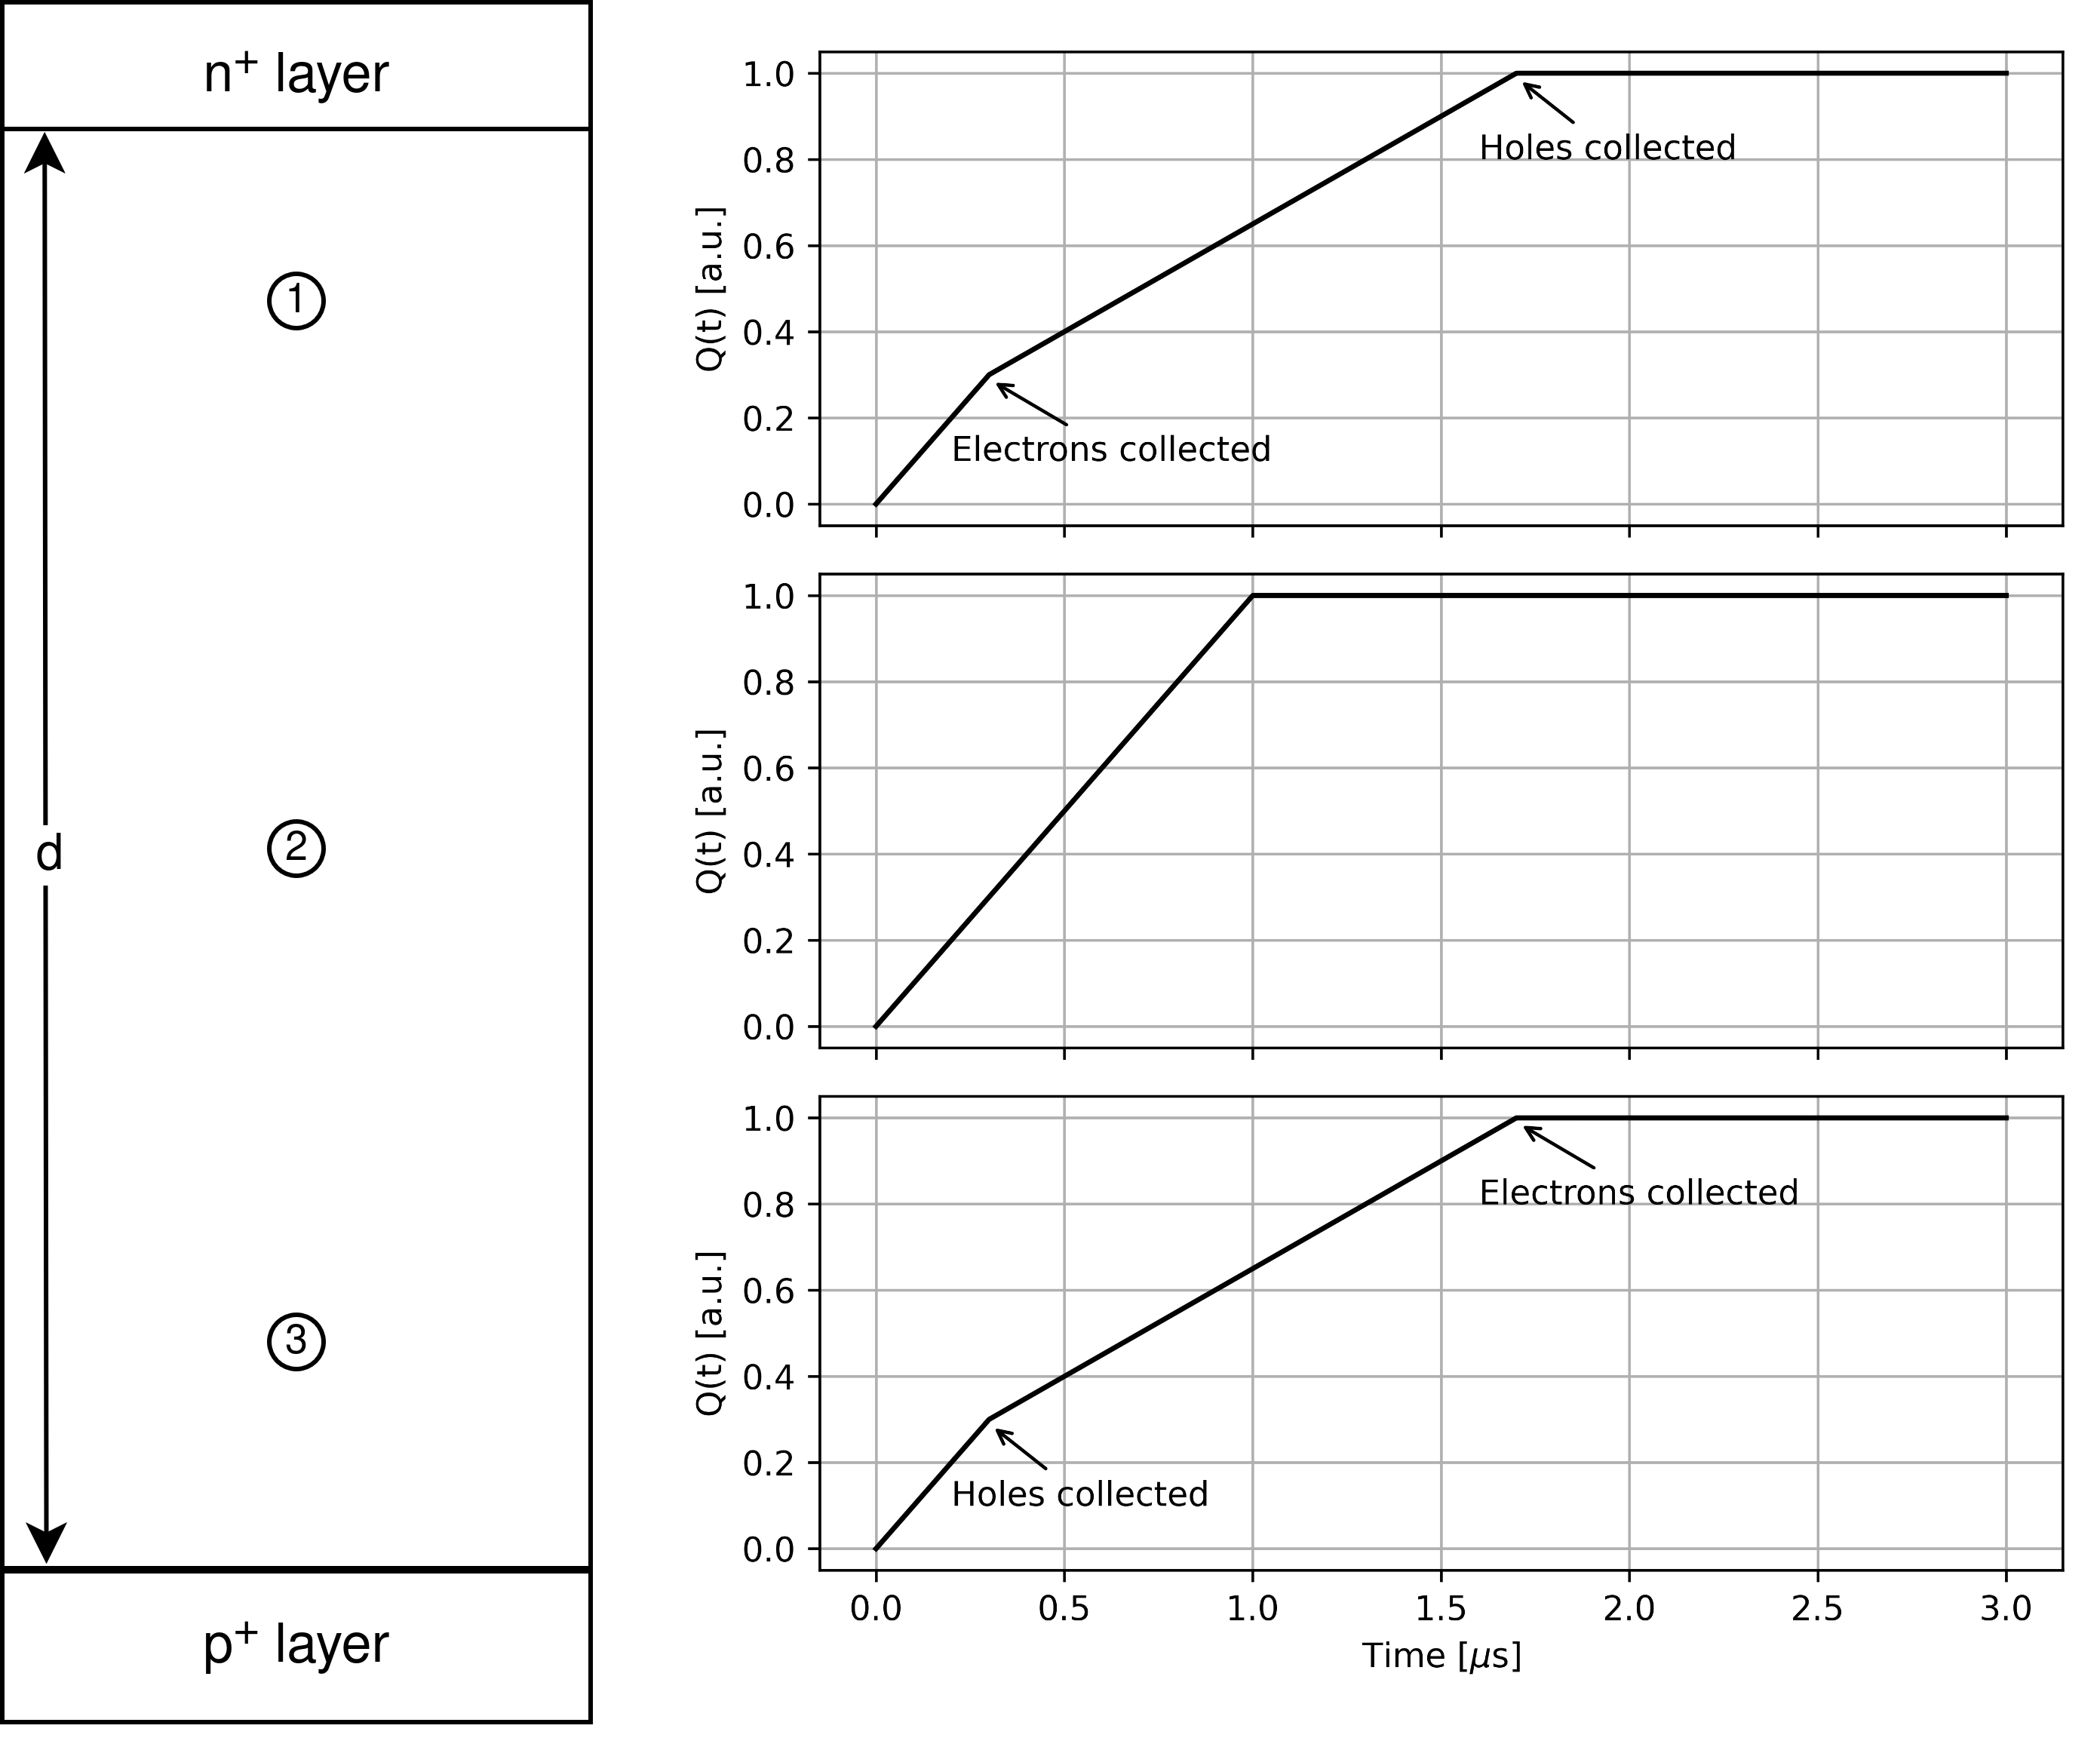
\includegraphics[width=0.85\linewidth]{figures/03_legend/Charge_collection_planar.png}
    \caption{Shape of the leading edge for three energy depositions inside a planar HPGe detector. Charge depositions close to the p$^+$ layer (bottom panel) are characterized by a very fast hole-induced signal, followed by a slower electron-induced signal, as the latter must drift across the entire detector volume. Similarly, charge depositions close to the n$^+$ layer are characterized by fast signals from the electrons, followed by a slower hole-induced signal. Here, we assume a detector of height $d=20$~cm and drift velocities of $10^{7}$~cm/s.}
\label{fig:Pulse_shape}
\end{figure}

In practice, however, signals recorded in HPGe detectors deviate from these idealized shapes due to additional effects that smooth out the signal. 
Crystal defects such as vacancies, dislocations, or impurities can locally trap charge carriers during their drift, preventing a fraction of the charge from reaching the electrodes. This reduces the signal amplitude and degrades energy resolution, as a variable amount of charge is lost.
Not all trapped carriers remain trapped permanently. Some are released after a time delay through de-trapping, which partially restores the signal but leads to a longer rise time. Both effects are illustrated in figure~\ref{fig:trapping_detrapping}~\cite{knoll_radiation_2000}. 


\begin{figure}
    \centering
    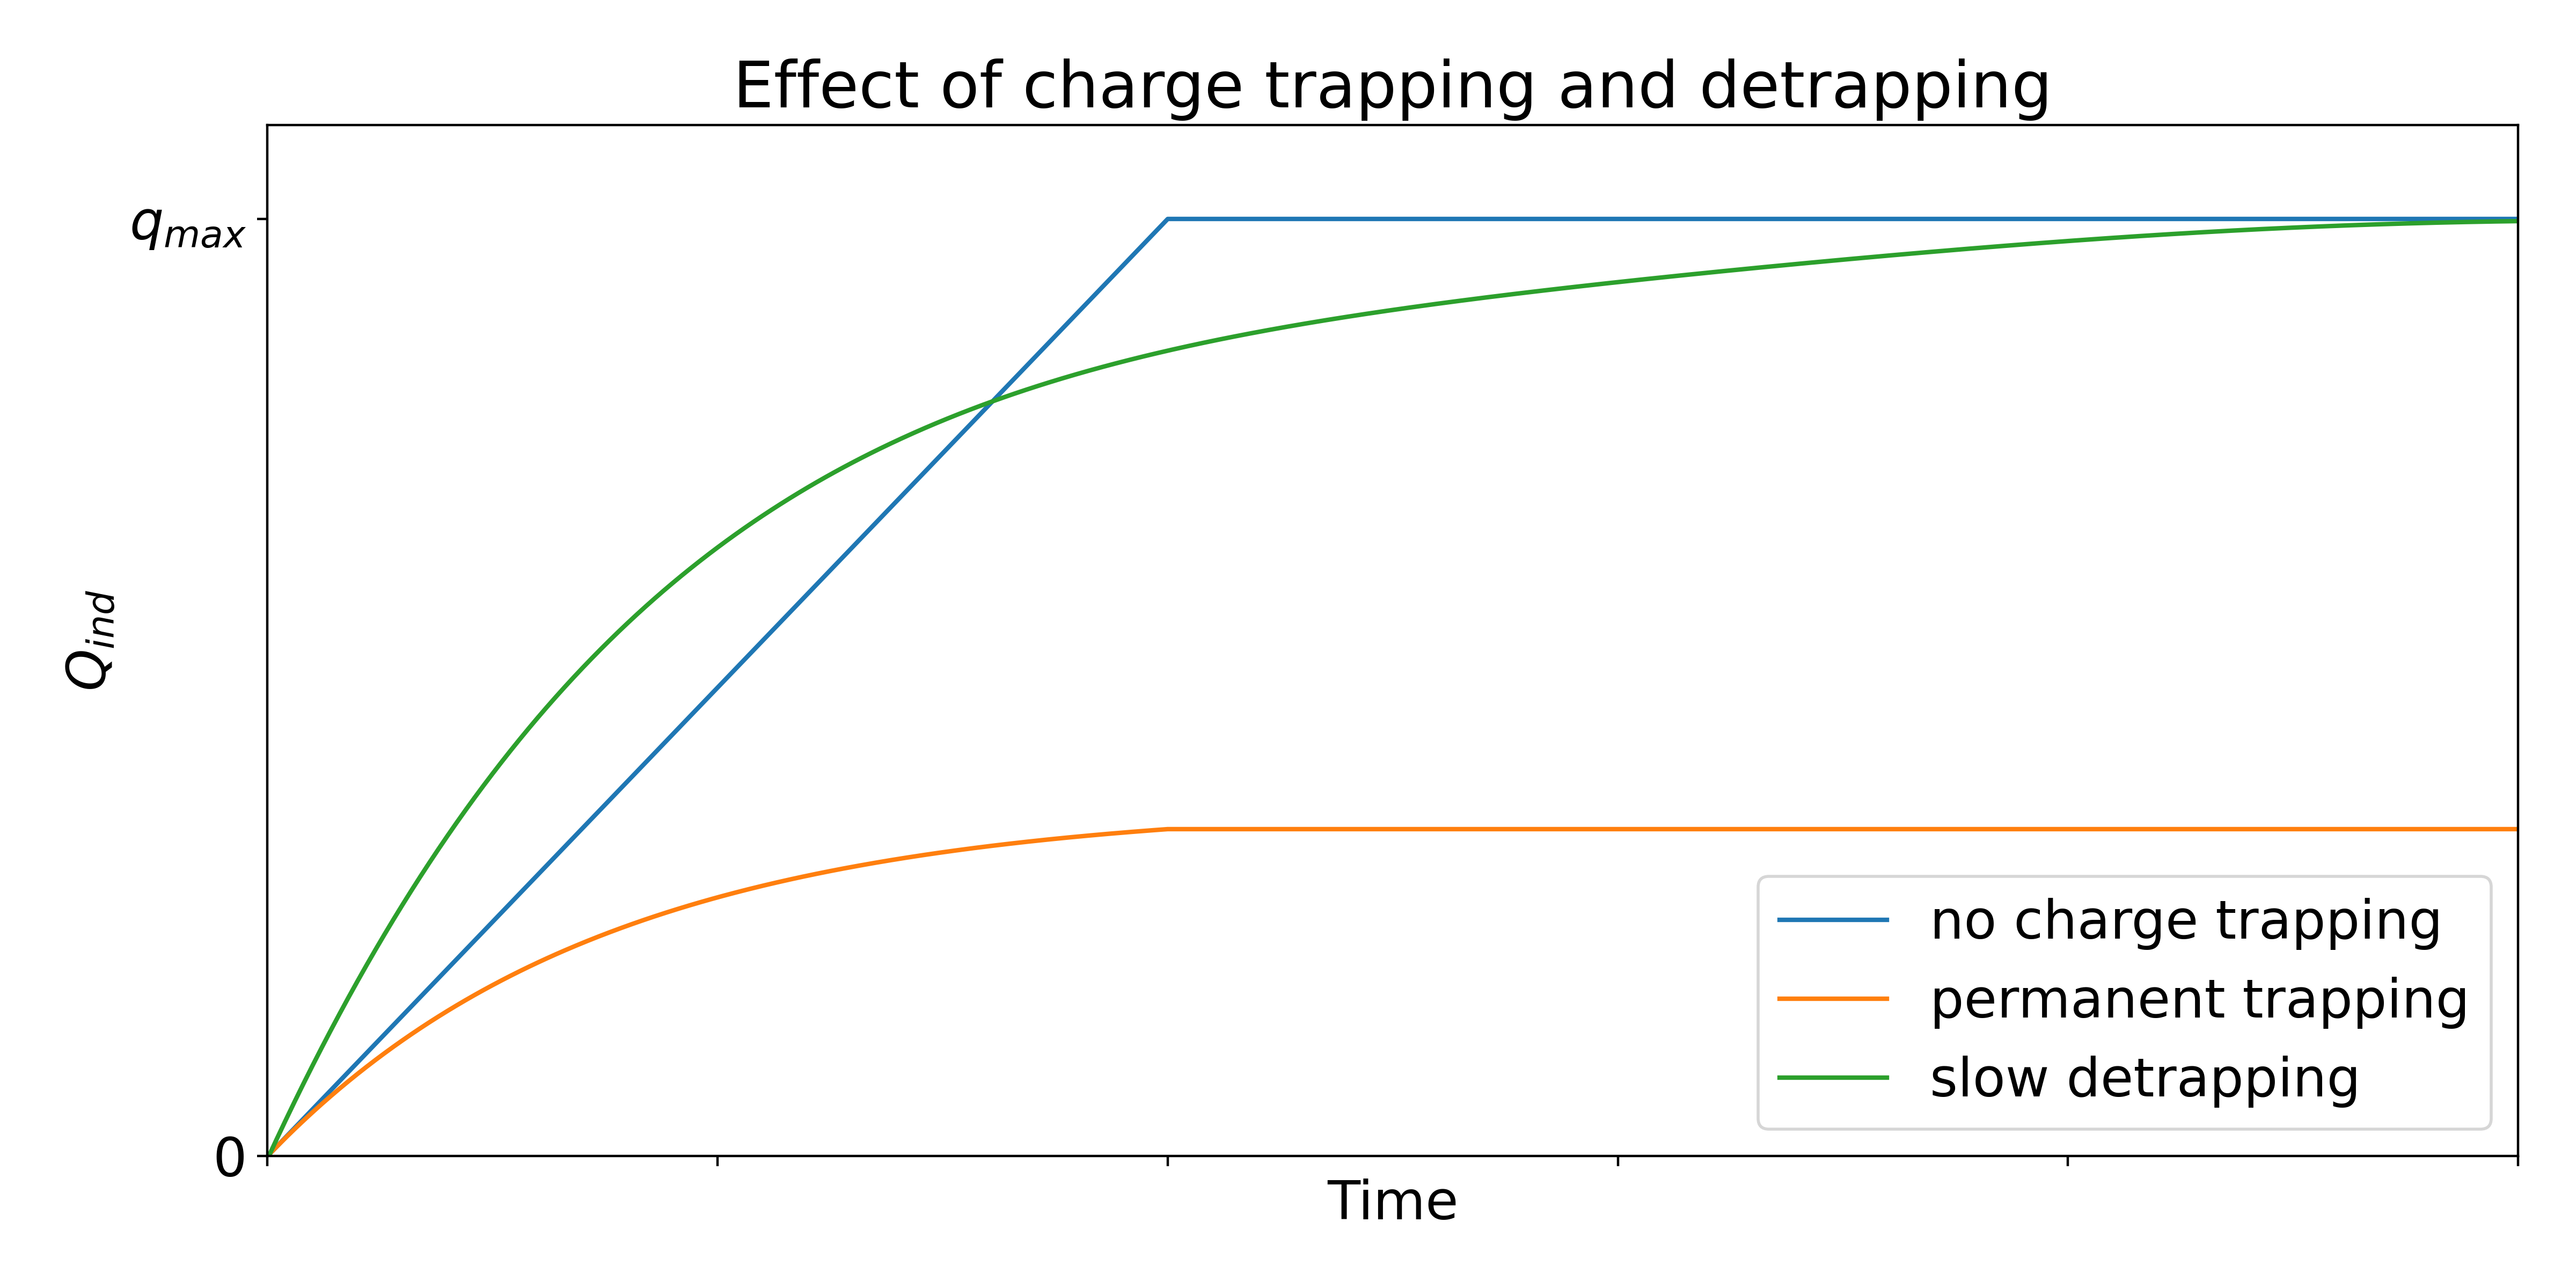
\includegraphics[width=0.75\linewidth]{figures/03_legend/Plot_charge_trapping.png}
    \caption{Effect of charge trapping and de-trapping on the rising edge of a HPGe waveform. Assuming a perfect semiconductor where no charge trapping occurs (blue line), all charges would arrive in a very short period of time, leading to a sharp edge when $q_{\mathrm{max}}$ is reached. On the other hand, permanent trapping would reduce the maximum amplitude. The combined effect of trapping and detrapping results in a smoothed waveform that rises quickly at first, then more slowly over time. For simplicity, only one type of charge carrier is shown. Adapted from~\cite{knoll_radiation_2000}.}
\label{fig:trapping_detrapping}
\end{figure}

Other physical effects further modify the waveform in similar ways: 
Self-repulsion and diffusion cause the charge carriers to spread out into a charge cloud, rather than moving as point-like. As a result, not all charges arrive at the electrode simultaneously, and the sharp edge at $q_{\mathrm{max}}$ becomes smoothed out.
Crystal anisotropy leads to non-uniform drift velocities, since the mobility of charge carriers depends on the orientation of the crystal axes. Table~\ref{tab:charge_mobility} shows electron and hole mobilities for different crystallographic axes, indicated by Miller indices. The charge carrier drift velocity $v_{e/h}$ is related to the mobility as:

\begin{equation}
\label{eq:velocity_mobility}
    v_{e/h} = \mu_{e/h} \cdot E \,,
\end{equation}

\noindent where the subscript indicates electrons and holes, respectively.

\begin{table}
\centering
\caption{Electron and hole mobilities for different crystal axes in germanium at 77~K. The axes are indicated by Miller indices~\cite{Abt_2023}.} 
\label{tab:charge_mobility}
\begin{tabular}{|c | c | c |}
	\hline
    \textbf{Crystal axis} & \textbf{$\mu_e$ [cm$^2$/(Vs)]} & \textbf{$\mu_h$ [cm$^2$/(Vs)]} \\
    \hline
    $\langle100\rangle$ & 38609 & 61824 \\
    \hline
    $\langle111\rangle$ & 38536  & 61215 \\ 
    \hline
\end{tabular}
\end{table}


\subsubsection{HPGe detectors in LEGEND-200}
\label{sec:HPGe_legend}
The LEGEND-200 experiment initially employed the majority of the enriched HPGe detectors that were previously manufactured, characterized, and operated in the GERDA and MJD experiments. GERDA primarily used broad energy germanium (BEGe) detectors, while MJD mainly used p-type point contact (PPC) detectors, where the main germanium crystal is p-doped. Both detector types are optimized for $0 \nu \beta \beta$ decay searches, offering excellent energy resolution, low background levels, and precise event reconstruction capabilities~\cite{collaboration_legend-1000_2021}. 
In later phases of both experiments, a new type of detector was introduced. The p-type inverted coaxial point contact (ICPC) detector allows for larger individual detector sizes while simultaneously increasing the pulse shape discrimination and energy resolution. Typical masses for these types are 1~kg for PPC, 0.7~kg for BEGe and 2-4~kg for ICPC detectors. 
For LEGEND-200, new ICPC detectors were developed and installed. Using larger detectors provides multiple advantages. Most importantly, it reduces the number of required cables, readout electronics, and mechanical support structures, all of which contribute to the overall background. 
Furthermore, a lower surface-to-volume ratio reduces the detector's sensitivity to surface-related backgrounds~\cite{collaboration_legend-1000_2021}. 

Traditional coaxial detectors, which were used in GERDA and have been installed in LEGEND-200 as well, do not offer the same level of performance as ICPC detectors. Consequently, they are not planned for use in future phases of LEGEND. In fact, the LEGEND collaboration will primarily rely on ICPC detectors moving forward. 
Figure~\ref{fig:legend_hpge_types} illustrates the three detector geometries. The layout of the LEGEND-200 detector array, as it was at the point of this work, is shown in figure~\ref{fig:legend_hpge_array}. 


\begin{figure}
    \centering
    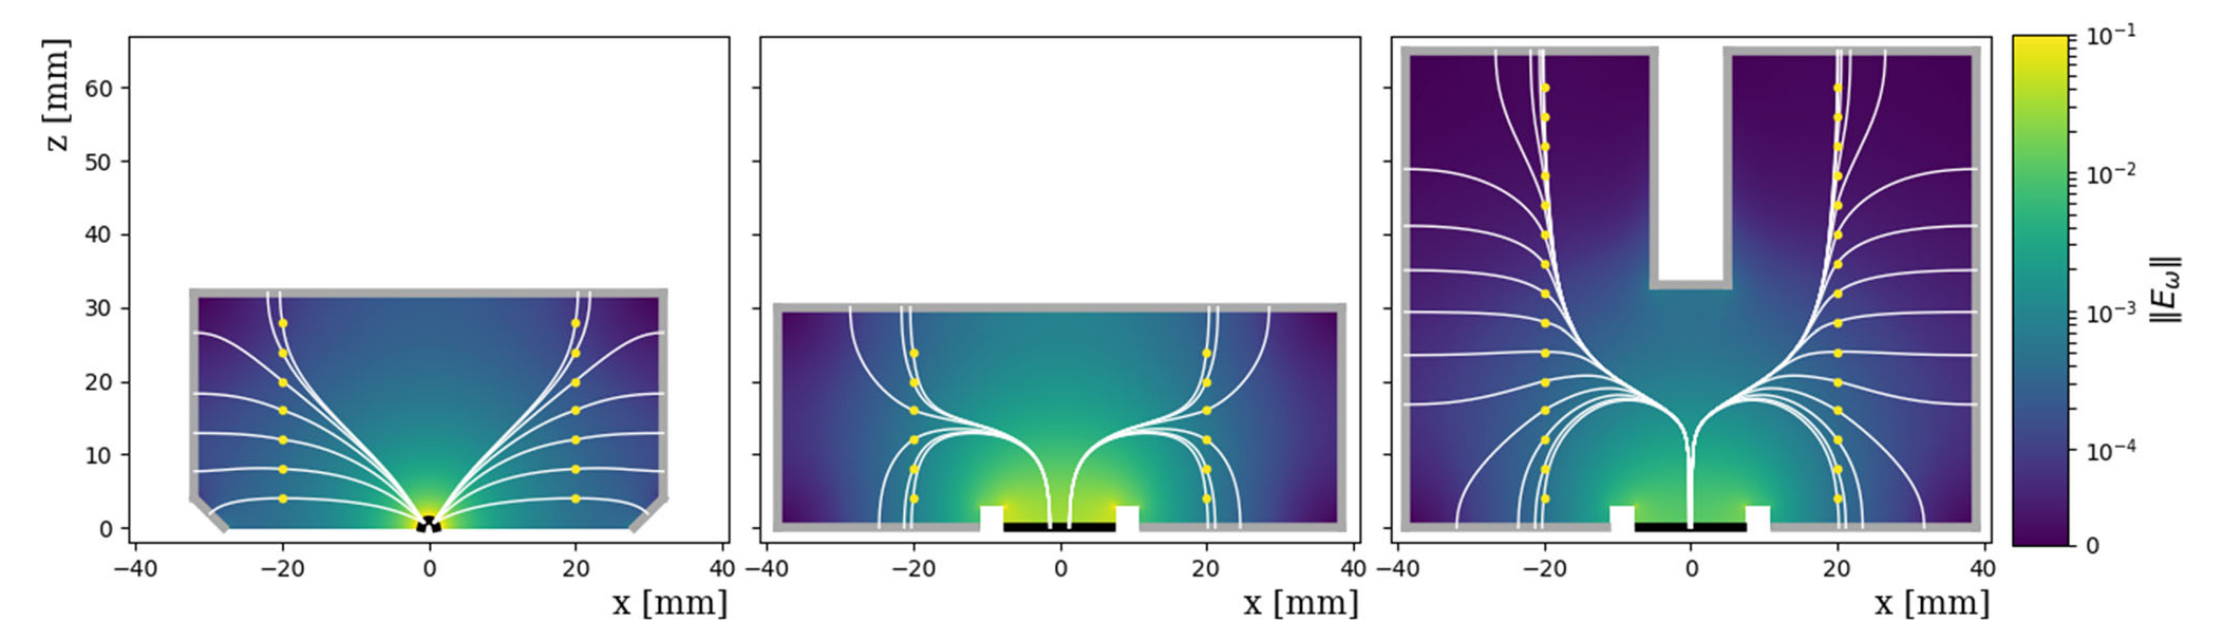
\includegraphics[width=1\linewidth]{figures/03_legend/Detectors_LEGEND.png}
    \caption{Cross section of three detector geometries used in LEGEND-200, including their respective weighting fields: PPC (left), BEGe (middle), and ICPC (right). The black line at the bottom indicates the p$^+$ contact, and the grey line surrounding the detector represents the n$^+$ electrode. Yellow dots mark exemplary interaction points, and white lines show the corresponding charge carrier trajectories. Plot from~\cite{collaboration_legend-1000_2021}.}
    \label{fig:legend_hpge_types}
\end{figure}



\begin{figure}[t]
    \centering
    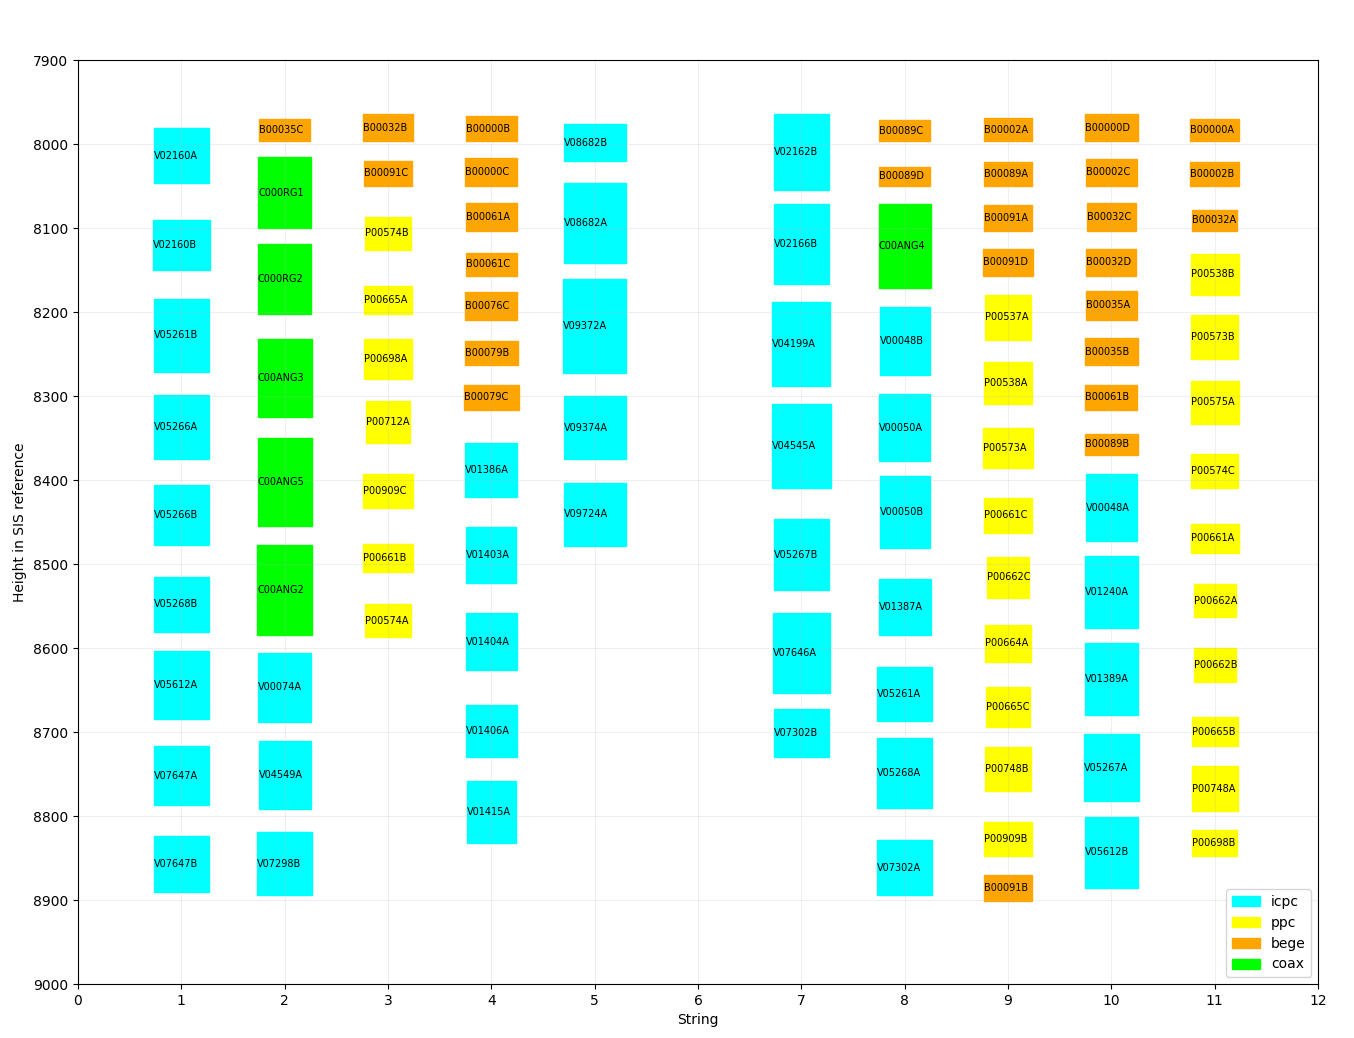
\includegraphics[width=0.95\linewidth]{figures/03_legend/improved_detector_arrangement_SGaelli.png}
    \caption{Detector map of the HPGe array installed in LEGEND-200. The germanium diodes are mounted on 11 strings. The y-axis indicates the vertical position relative to the top of the detector, where the source insertion system is located. The colors indicate the different detector geometries. ICPC detectors are blue, PPC detectors are yellow, BEGe detectors are orange and the coaxial detectors are indicated in green. Image credits of Sandro Gaelli.}
    \label{fig:legend_hpge_array}
\end{figure}



The detectors used in LEGEND-200 are all p-type HPGe diodes, equipped with a relatively thin ($\sim$ 300~nm) p$^+$ electrode that is formed via boron implantation. The n$^+$ electrode, doped with lithium, is significantly thicker ($\sim$ 1-2~mm) and covers most of the detector surface~\cite{agostini_pulse_2022}. The signal is read out from the small p$^+$ electrode, because the charge signal is dominated by hole drift in this geometry. 

In LEGEND-200, detector signals are processed by a two-stage resistive-feedback charge-sensitive amplifier (CSA) operated in liquid argon for cooling and radiopurity. 
The Low-Mass Front End is mounted only millimeters from each HPGe detector, using ultra-radiopure materials and a high-value amorphous-germanium feedback resistor. A differential amplifier, positioned 30–150 cm away, boosts the signal for transmission to the data acquisition (DAQ) system. This design achieves electronic noise equivalent to $< 1$~keV FWHM, energy resolution of $\leq 2.5$~keV at $Q_{\beta \beta}$, and fast ($\leq 100$~ns) rise times, enabling precise energy reconstruction and effective pulse-shape discrimination~\cite{Willers_2020}.

The DAQ system reads out the signals at a rate of 62.5~MHz, corresponding to a sampling interval of 16~ns. This is sufficiently fast to resolve the characteristic signal rise times. The digitized waveform is a voltage step with an exponential decay from the feedback circuit and superimposed electronic noise, and therefore requires further processing.

The digital processing begins with a baseline subtraction and pole-zero cancellation to remove the exponential decay, yielding an idealized step. The resulting waveform is then step-like. The signal is then shaped using a trapezoidal (trap) filter, implemented by subtracting two moving averages of different widths to produce a waveform with a defined rise, flat top, and fall. The flat top is rounded via additional moving averages to yield a single, well-defined maximum. The amplitude is taken as this maximum, and its value is proportional to the collected charge~\cite{Willers_2020, salathe_2016150}.  


\subsection{Calibration of the LEGEND-200 experiment}

A successful search for $0 \nu \beta \beta$ decay requires excellent energy resolution and a stable energy scale, which in turn requires regular calibration of every detector.
After digital signal processing, the waveform remains in units of ADC counts. To convert these into physical energy, radioactive sources with a well-known $\gamma$ spectrum are periodically inserted into the cryostat using an automated source insertion system (SIS). This is necessary because the isotope used for LEGEND-200, as well as GERDA and MJD, $^{228}$Th, has a relatively short half-life of 1.9~years~\cite{collaboration_legend-1000_2021}.
The SIS allows sources to be inserted for calibration runs and removed during physics data-taking. Sources are guided near the detector strings through dedicated copper funnels, which are required to navigate the sources to their calibration positions next to the detectors. LEGEND-200 comprises four SIS, each accommodating four sources~\cite{mueller2023}. 

Once sufficient statistics are collected, the resulting $\gamma$ lines appear in the energy histogram; matching their known energies to the measured ADC positions yields the calibration curve. 
In addition to determining the absolute energy scale, calibration is essential for evaluating the detector's energy resolution. This is critical for $0 \nu \beta \beta$ searches, as a precise determination of the peak at $Q_{\beta \beta}$ with a high resolution is necessary for effective background discrimination and therefore maximizing signal sensitivity.  

$^{228}$Th decays through a series of $\alpha$ and $\beta$ transitions to $^{208}$Pb, emitting several characteristic $\gamma$ rays along the way~\cite{baudis_calibration_2023}. The decay scheme is shown in figure~\ref{fig:Th228_decay_chain}. 

\begin{figure}
    \centering
    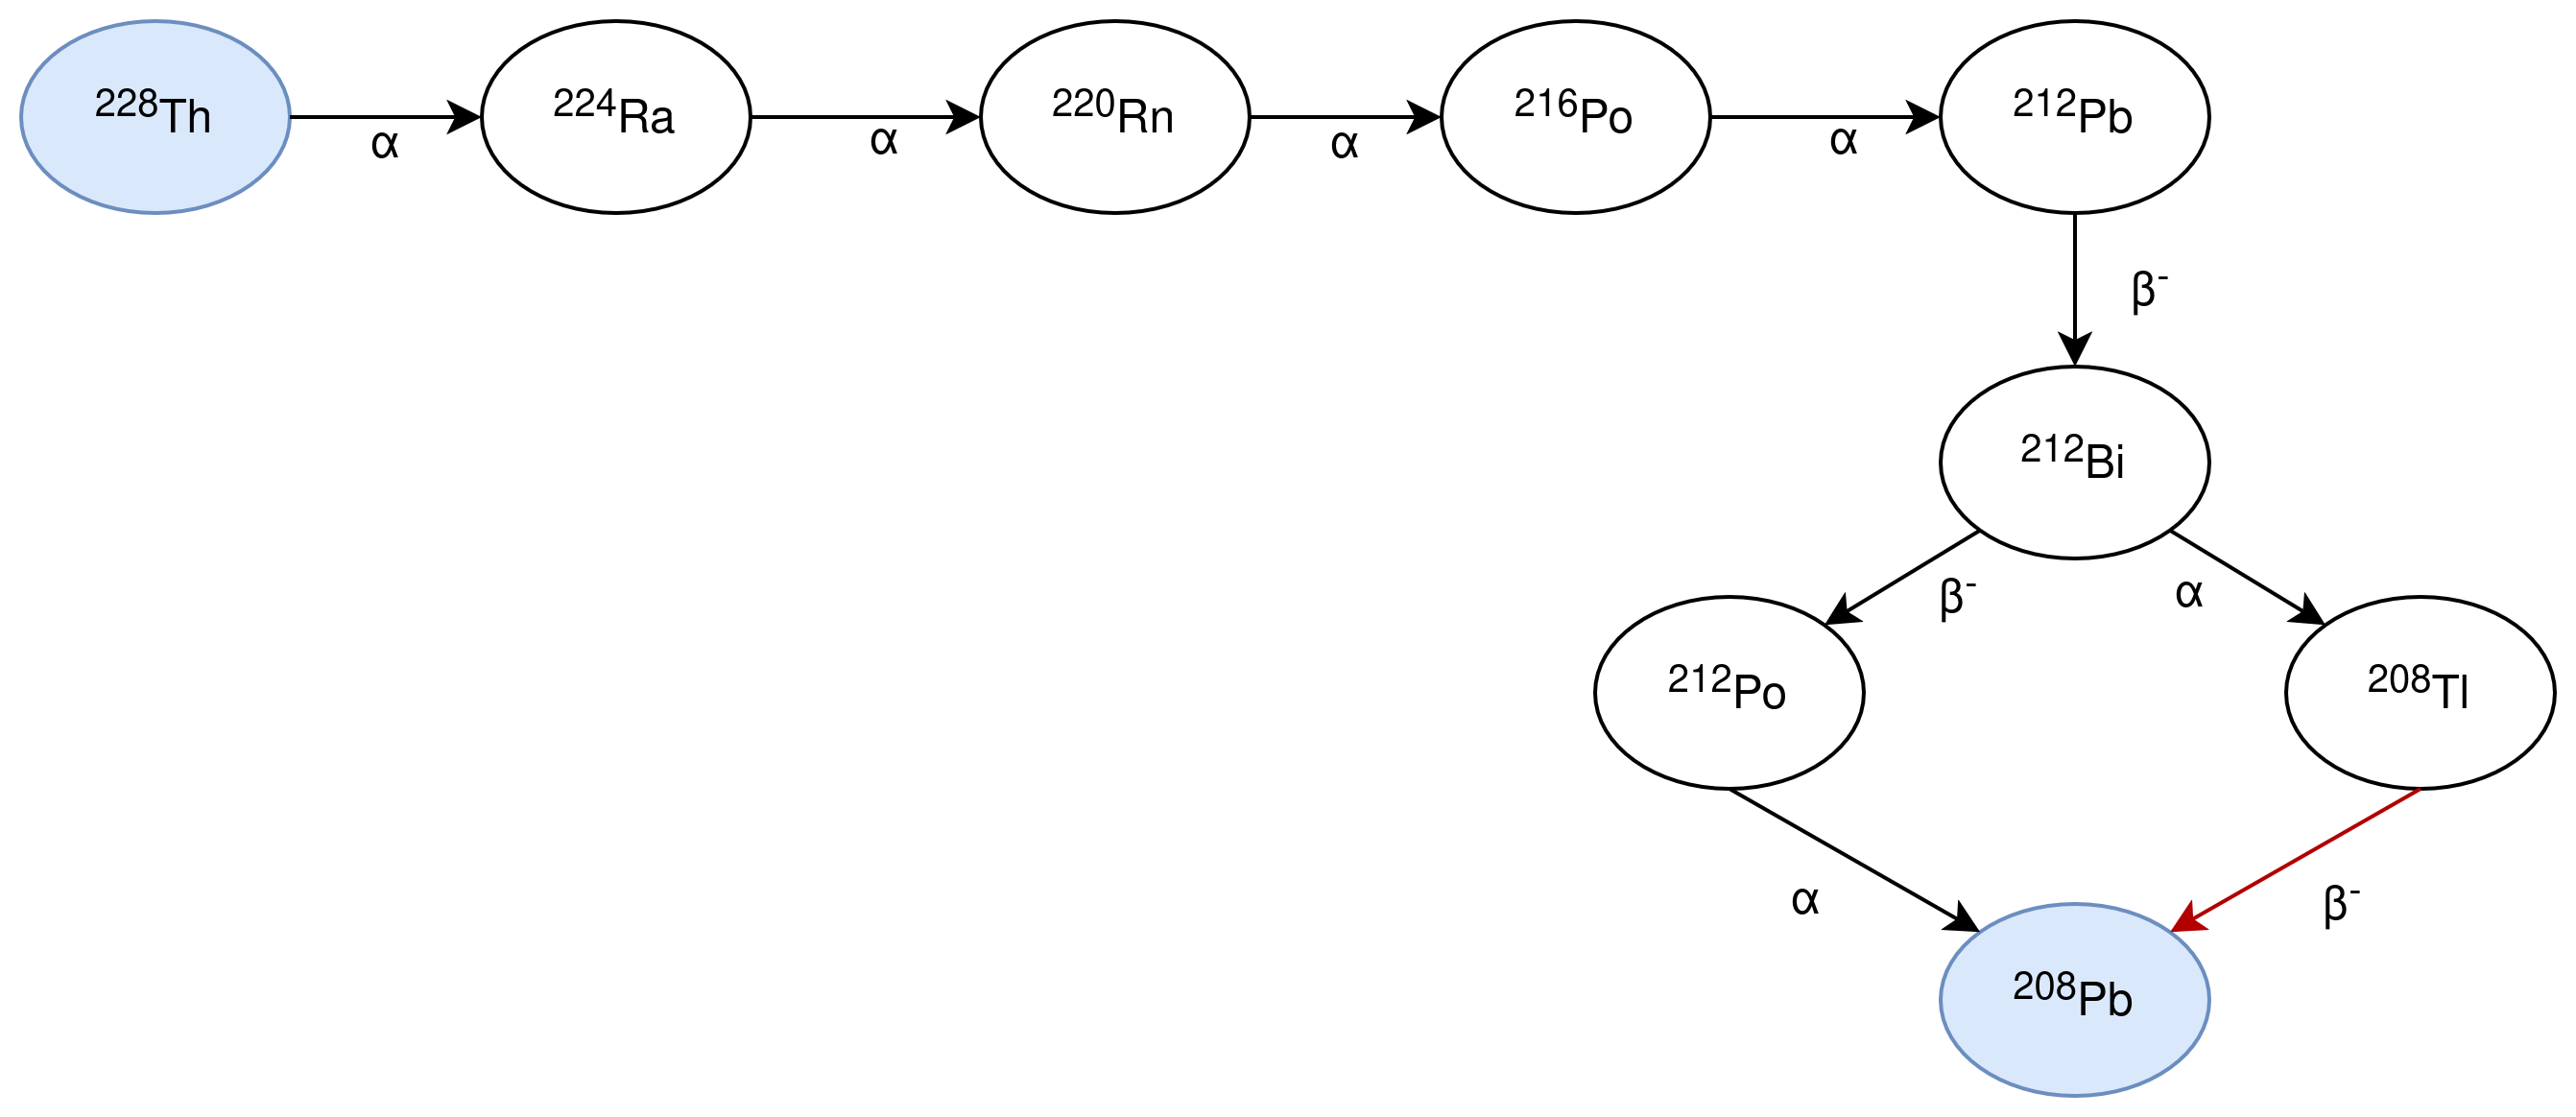
\includegraphics[width=\linewidth]{figures/03_legend/Th228_decay_chain.png}
    \caption{Decay chain of $^{228}$Th to $^{208}$Pb. For energy calibration and pulse shape studies, the $\beta^-$ decay of $^{208}$Tl is most important, because it produces several $\gamma$ lines used for calibration. This decay is indicated by the red arrow.}
    \label{fig:Th228_decay_chain}
\end{figure}

The most important line is the $^{208}$Tl 2614.5 keV $\gamma$. When this photon undergoes pair production inside a HPGe detector, the resulting electron deposits its kinetic energy, and the positron annihilates into two 511 keV photons. Depending on whether none, one, or both annihilation photons escape, three distinct peaks appear: 

\noindent \textbf{Full-energy peak} (2614.5 keV): No photons escape, and the waveform contains multiple events. 

\noindent \textbf{Single-escape peak} (2103.5 keV): One photon escapes, there are still multiple events per waveform due to the time separation between deposits. 

\noindent \textbf{Double-escape peak} (1592.5 keV): Both photons escape, and the remaining energy deposition is highly localized and thus single-site~\cite{baudis_calibration_2023, agostini_pulse_2022}.

A further useful line is the $^{212}$Bi full-energy peak at 1621 keV. Its proximity to the double-escape peak makes it convenient for energy-independent comparisons of single-site and multi-site populations~\cite{agostini_pulse_2022}. Figure~\ref{fig:Calibration_spectrum_Th228} shows a representative $^{228}$Th calibration spectrum recorded with a single ICPC detector in LEGEND-200, with the key peaks highlighted.   


\begin{figure}
    \centering
    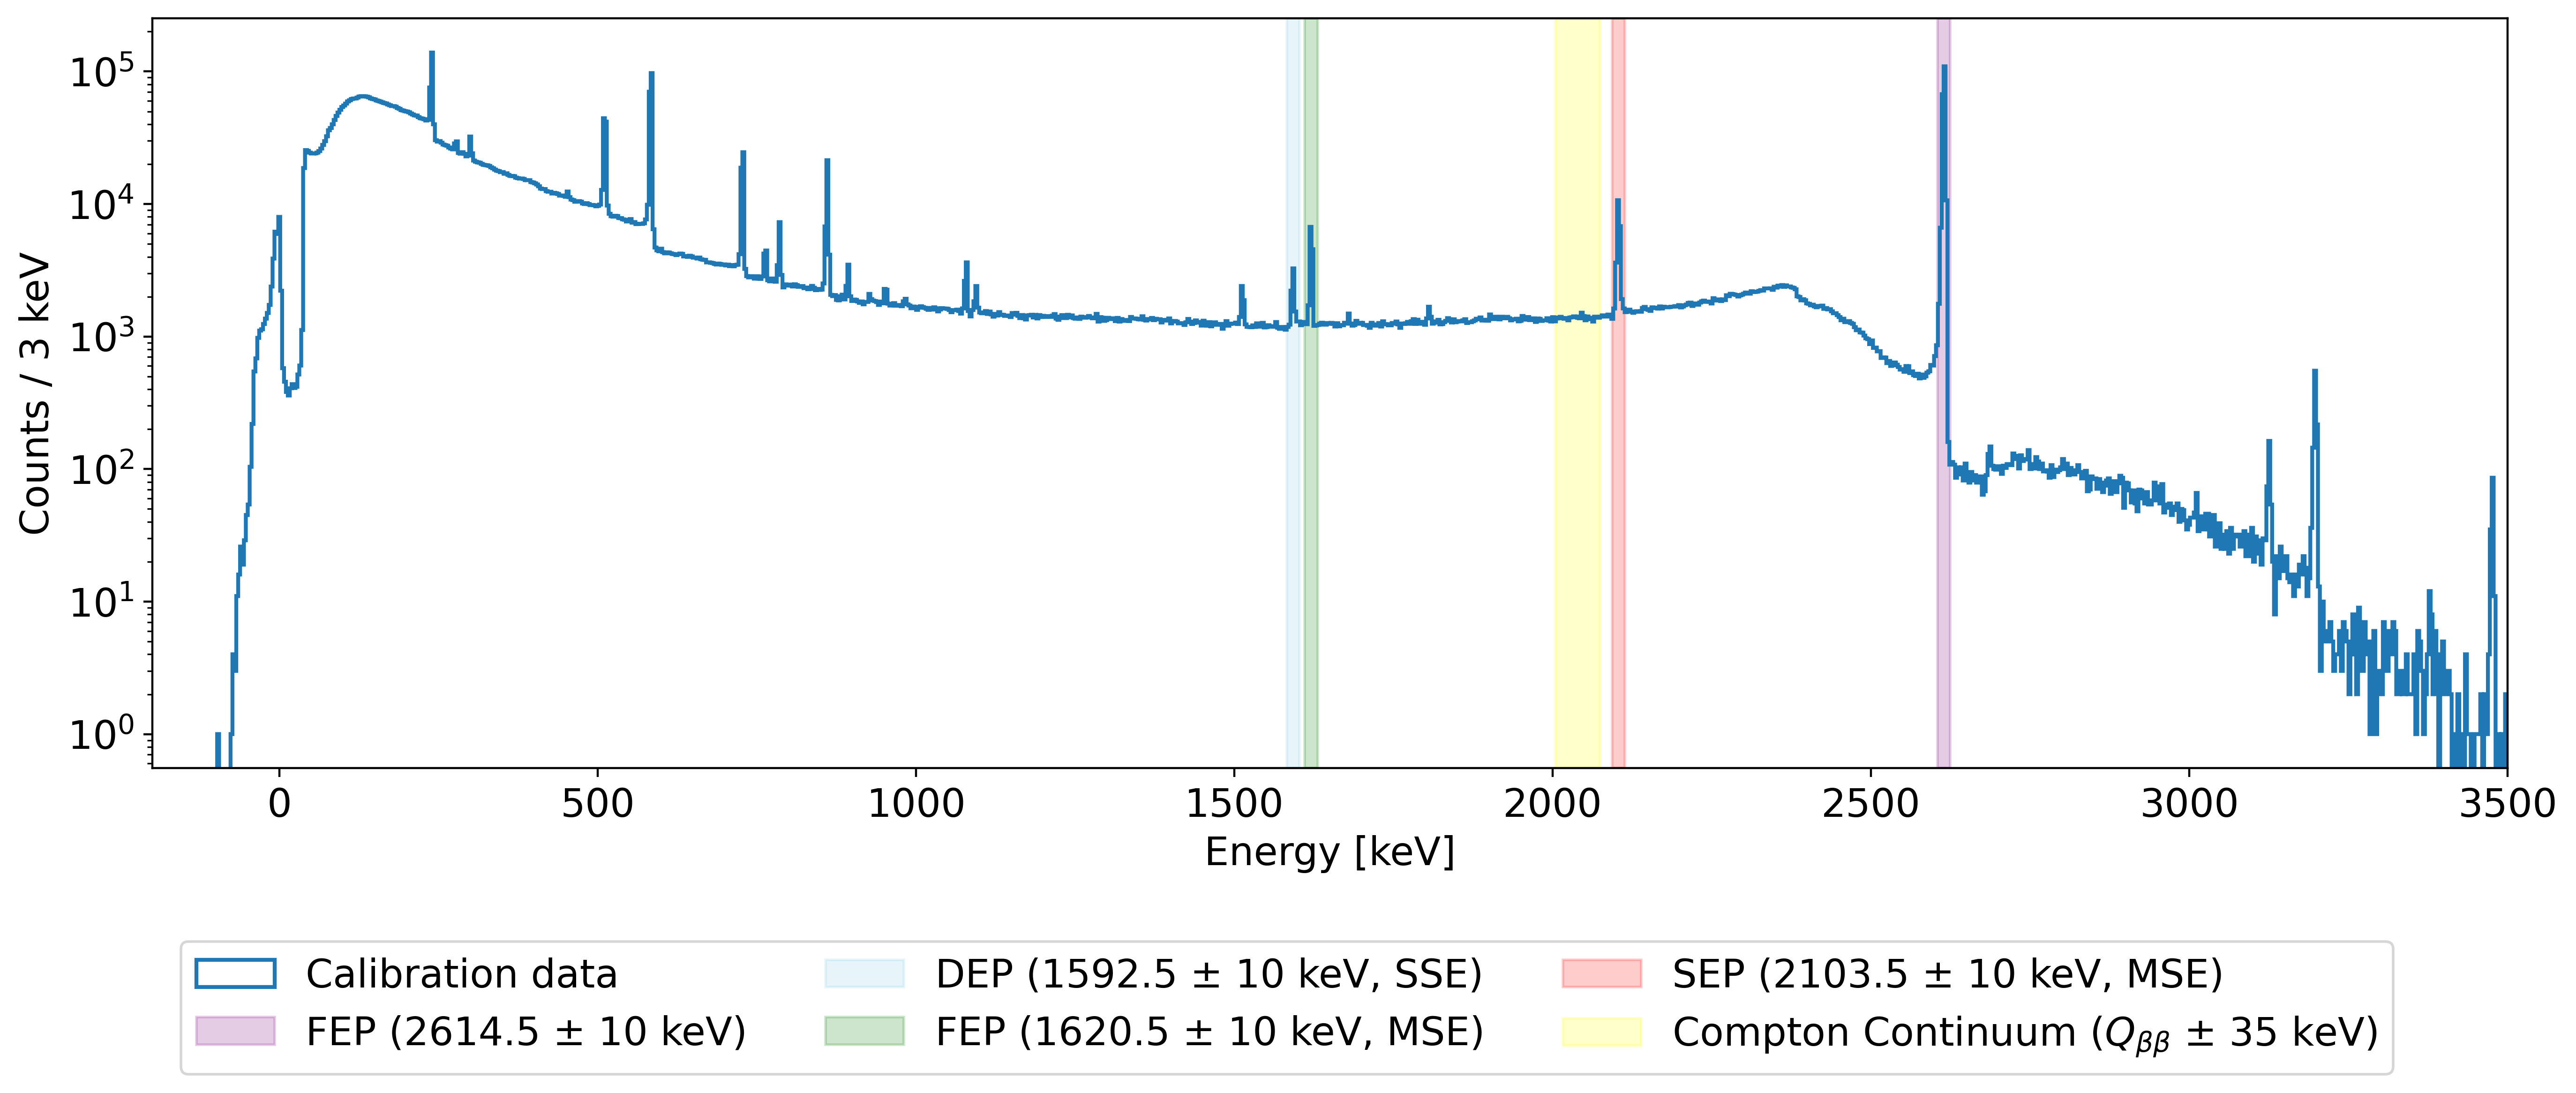
\includegraphics[width=\linewidth]{figures/03_legend/Calibration_spectrum_Th228_V09372A.png}
    \caption{Energy spectrum from a $^{228}$Th calibration run (period 9, run 3) in LEGEND-200. The spectrum corresponds to a single IC detector (V09372A) and a 5-hour data acquisition. Prominent $\gamma$-ray lines used for calibration and PSD studies are indicated.}
    \label{fig:Calibration_spectrum_Th228}
\end{figure}


In addition to $^{228}$Th, LEGEND also recorded data with a $^{56}$Co source. It is not used for detector calibration, but since it emits several $\gamma$ lines at energies that complement those of $^{228}$Th, it is a valuable source for studying the energy dependence of the PSD efficiency. 


\subsection{Background rejection: pulse shape discrimination}
\label{sec:02_PSD}

Even with large detector masses and multi-year exposures, only a handful of $0 \nu \beta \beta$ decay events are to be expected. At the same time, numerous background processes can deposit energy in the region of interest around $Q_{\beta \beta} = 2039$~keV.
Without effective background rejection methods, these events would obscure the $0\nu\beta\beta$ signal entirely. Moreover, as shown in equation~\refeq{eq:0vbb_hl_sensitivity}, the experimental sensitivity to the half-life scales inversely with the square root of the background index, meaning that lowering the background significantly improves sensitivity. 
Background rejection in LEGEND is achieved through a combination of material selection, active veto systems, and signal-based analysis techniques. Of particular importance for this work is pulse shape discrimination, which is possible because HPGe detectors record ionization signals with high temporal and spatial precision.
In LEGEND, we distinguish between four characteristic pulse shapes: 


\textbf{Single-site events (SSE)} are characterized by very localized energy depositions. This applies to both $0 \nu \beta \beta$ and $2 \nu \beta \beta$ decays, where the electrons deposit their energy within a small volume (typically $\sim 1$~mm$^3$). The resulting charges drift to the electrodes nearly simultaneously, and the waveform resembles that of a single interaction.

\textbf{Multi-site events (MSE)} involve energy deposited at multiple locations, typically due to multiple Compton scatterings of high-energy $\gamma$ rays from natural radioactivity. These events are classified as background in the context of neutrinoless double beta decay. 

Surface events occur near the detector boundaries and are also associated with the background. \textbf{P-contact events}, such as $\alpha$ interactions near the p$^{+}$ electrode, produce a fast-rising signal, since the drift path is short. Such surface events are particularly dangerous because their localized energy deposition can mimic the topology of SSEs, but their distorted charge collection leads to subtle differences in the pulse shape that must be carefully identified and rejected. 
In contrast, \textbf{n-contact events}, which originate near the $n^{+}$ electrode, involve long drift paths for the holes through the entire detector. These signals tend to rise more slowly and may show distortions due to trapping, de-trapping, or charge loss in the dead layer.


\begin{figure}[t]
    \centering
    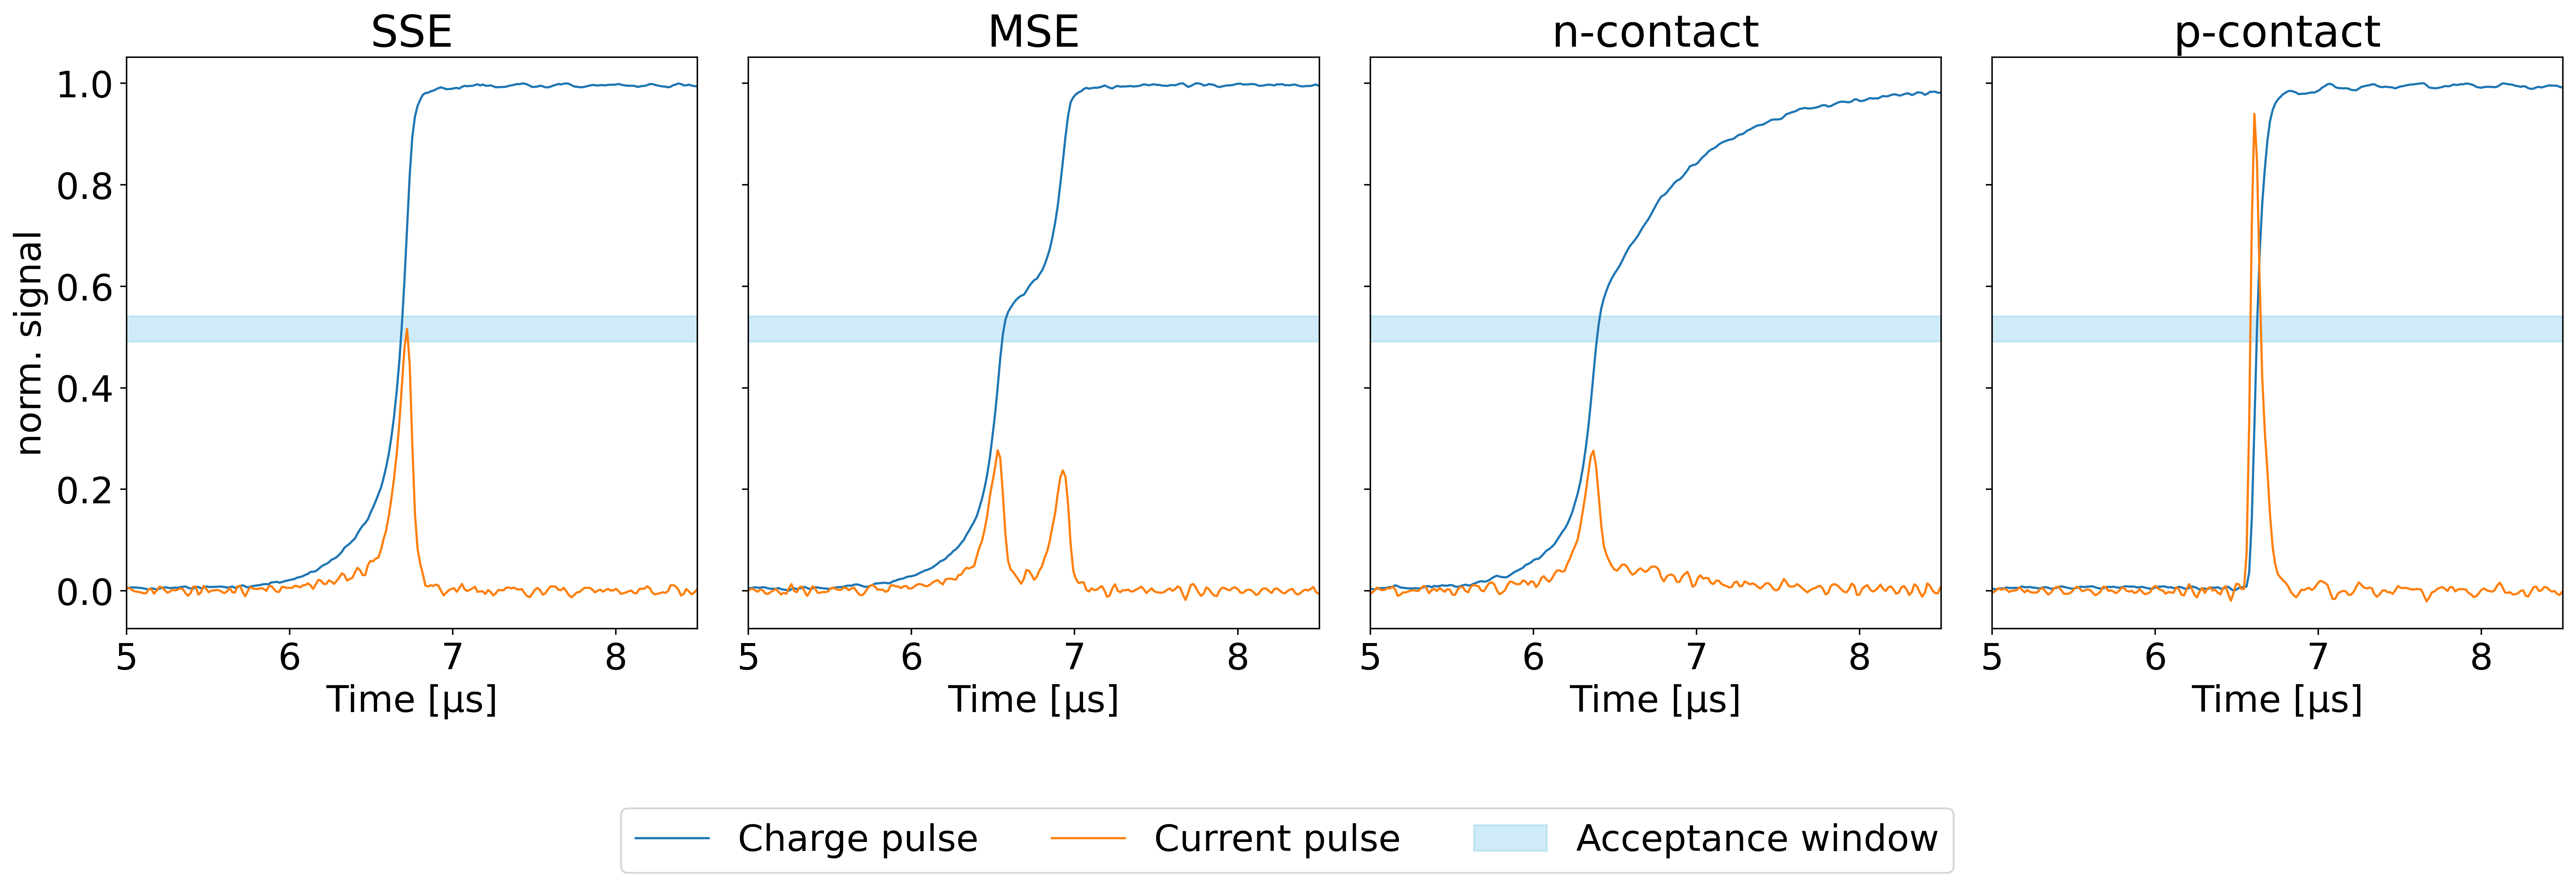
\includegraphics[width=\linewidth]{figures/03_legend/PSD_topology.png}
    \caption{Example waveforms from a $^{228}$Th calibration run in LEGEND-200, showing the normalized induced charge and corresponding current signal for four different event types. All examples have the same total deposited energy. The blue band illustrates, schematically, the A/E acceptance window for SSE-like signals; it is not derived from a quantitative cut but serves to illustrate the idea.}
    \label{fig:PSD_topology}
\end{figure}

Figure~\ref{fig:PSD_topology} illustrates these event types.
The standard PSD parameter is the amplitude over energy ratio (A/E), also referred to as AoE. Here, $A$ denotes the maximum of the waveform and $E$ is the reconstructed event energy, expressed in~keV after energy calibration. The A/E parameter is sensitive to the event topology: in SSE, all the energy is deposited in a localized volume, leading to a short charge collection time and thus a sharply peaked current pulse. In MSE, the energy is deposited in several locations, resulting in less peaked current pulses and smaller A/E ratios. 

The A/E distribution is calibrated by performing peak fits on $^{228}$Th calibration data. In the Compton bands, the A/E distribution is characterized by a Gaussian single-site band with a low-side tail from MSE and $n^{+}$ surface events. A high-energy tail accounts for $p^{+}$ surface events. The tails are modelled as an exponential distribution convolved with a Gaussian. 

Two corrections are applied. The A/E parameter depends on the drift time and the energy. Charge clouds drifting through the detector are subject to diffusion, which broadens the current signal. The A/E energy dependence is modelled as:

\begin{align}
\label{eq:AoE_energydep_mu}
\mu_{\mathrm{A/E}}(E) & = a + b \cdot E \\
\sigma_{\mathrm{A/E}}(E) & = \sqrt{c + \frac{d}{E^2}}
\label{eq:AoE_energydep_sigma} \,,
\end{align}

\noindent where $a,b,c,d$ are determined from calibration data in the Compton region from 900~keV to 2300~keV.  
For uniformity across detectors and calibration periods, a normalized A/E classifier is defined:


\begin{equation}
\label{eq:AoE_Classifier}
A/E_{\mathrm{classifier}} = \frac{\frac{A/E}{\mu_{A/E}(E) - 1}}{\sigma_{A/E}(E)} \,.
\end{equation}

This normalization accounts for detector-specific and time-dependent variations in the A/E response, enabling a unified classifier scale that allows consistent pulse shape discrimination across all detectors and calibration periods~\cite{lnote_24013}.


To isolate single-site events, two cut values are applied. 
The lower cut, which removes multi-site and n-contact events, is chosen such that 90\% of events in the $^{208}$Tl DEP survive. The upper cut is fixed to exclude high-amplitude surface events, in particular, $\alpha$ interactions~\cite{agostini_pulse_2022}.

The Late Charge (LQ) is a PSD parameter that measures the slowness of the final 20\% of charge carriers for an event. It is defined as the area above the rising edge of the waveform after it reaches 80\% of its maximum value. It is a powerful discriminator to identify events with slow charge collection, such as $p^{+}$ contact surface $\alpha$ interactions or events affected by significant charge trapping. 
Like the A/E parameter, the LQ parameter is both drift-time and energy dependent, and needs to be corrected for~\cite{lnote_24013}. 
The A/E and LQ distributions as functions of energy for a single IC detector are shown in figure~\ref{fig:Aoe_LQ_spectra}. 

\begin{figure}
    \centering
    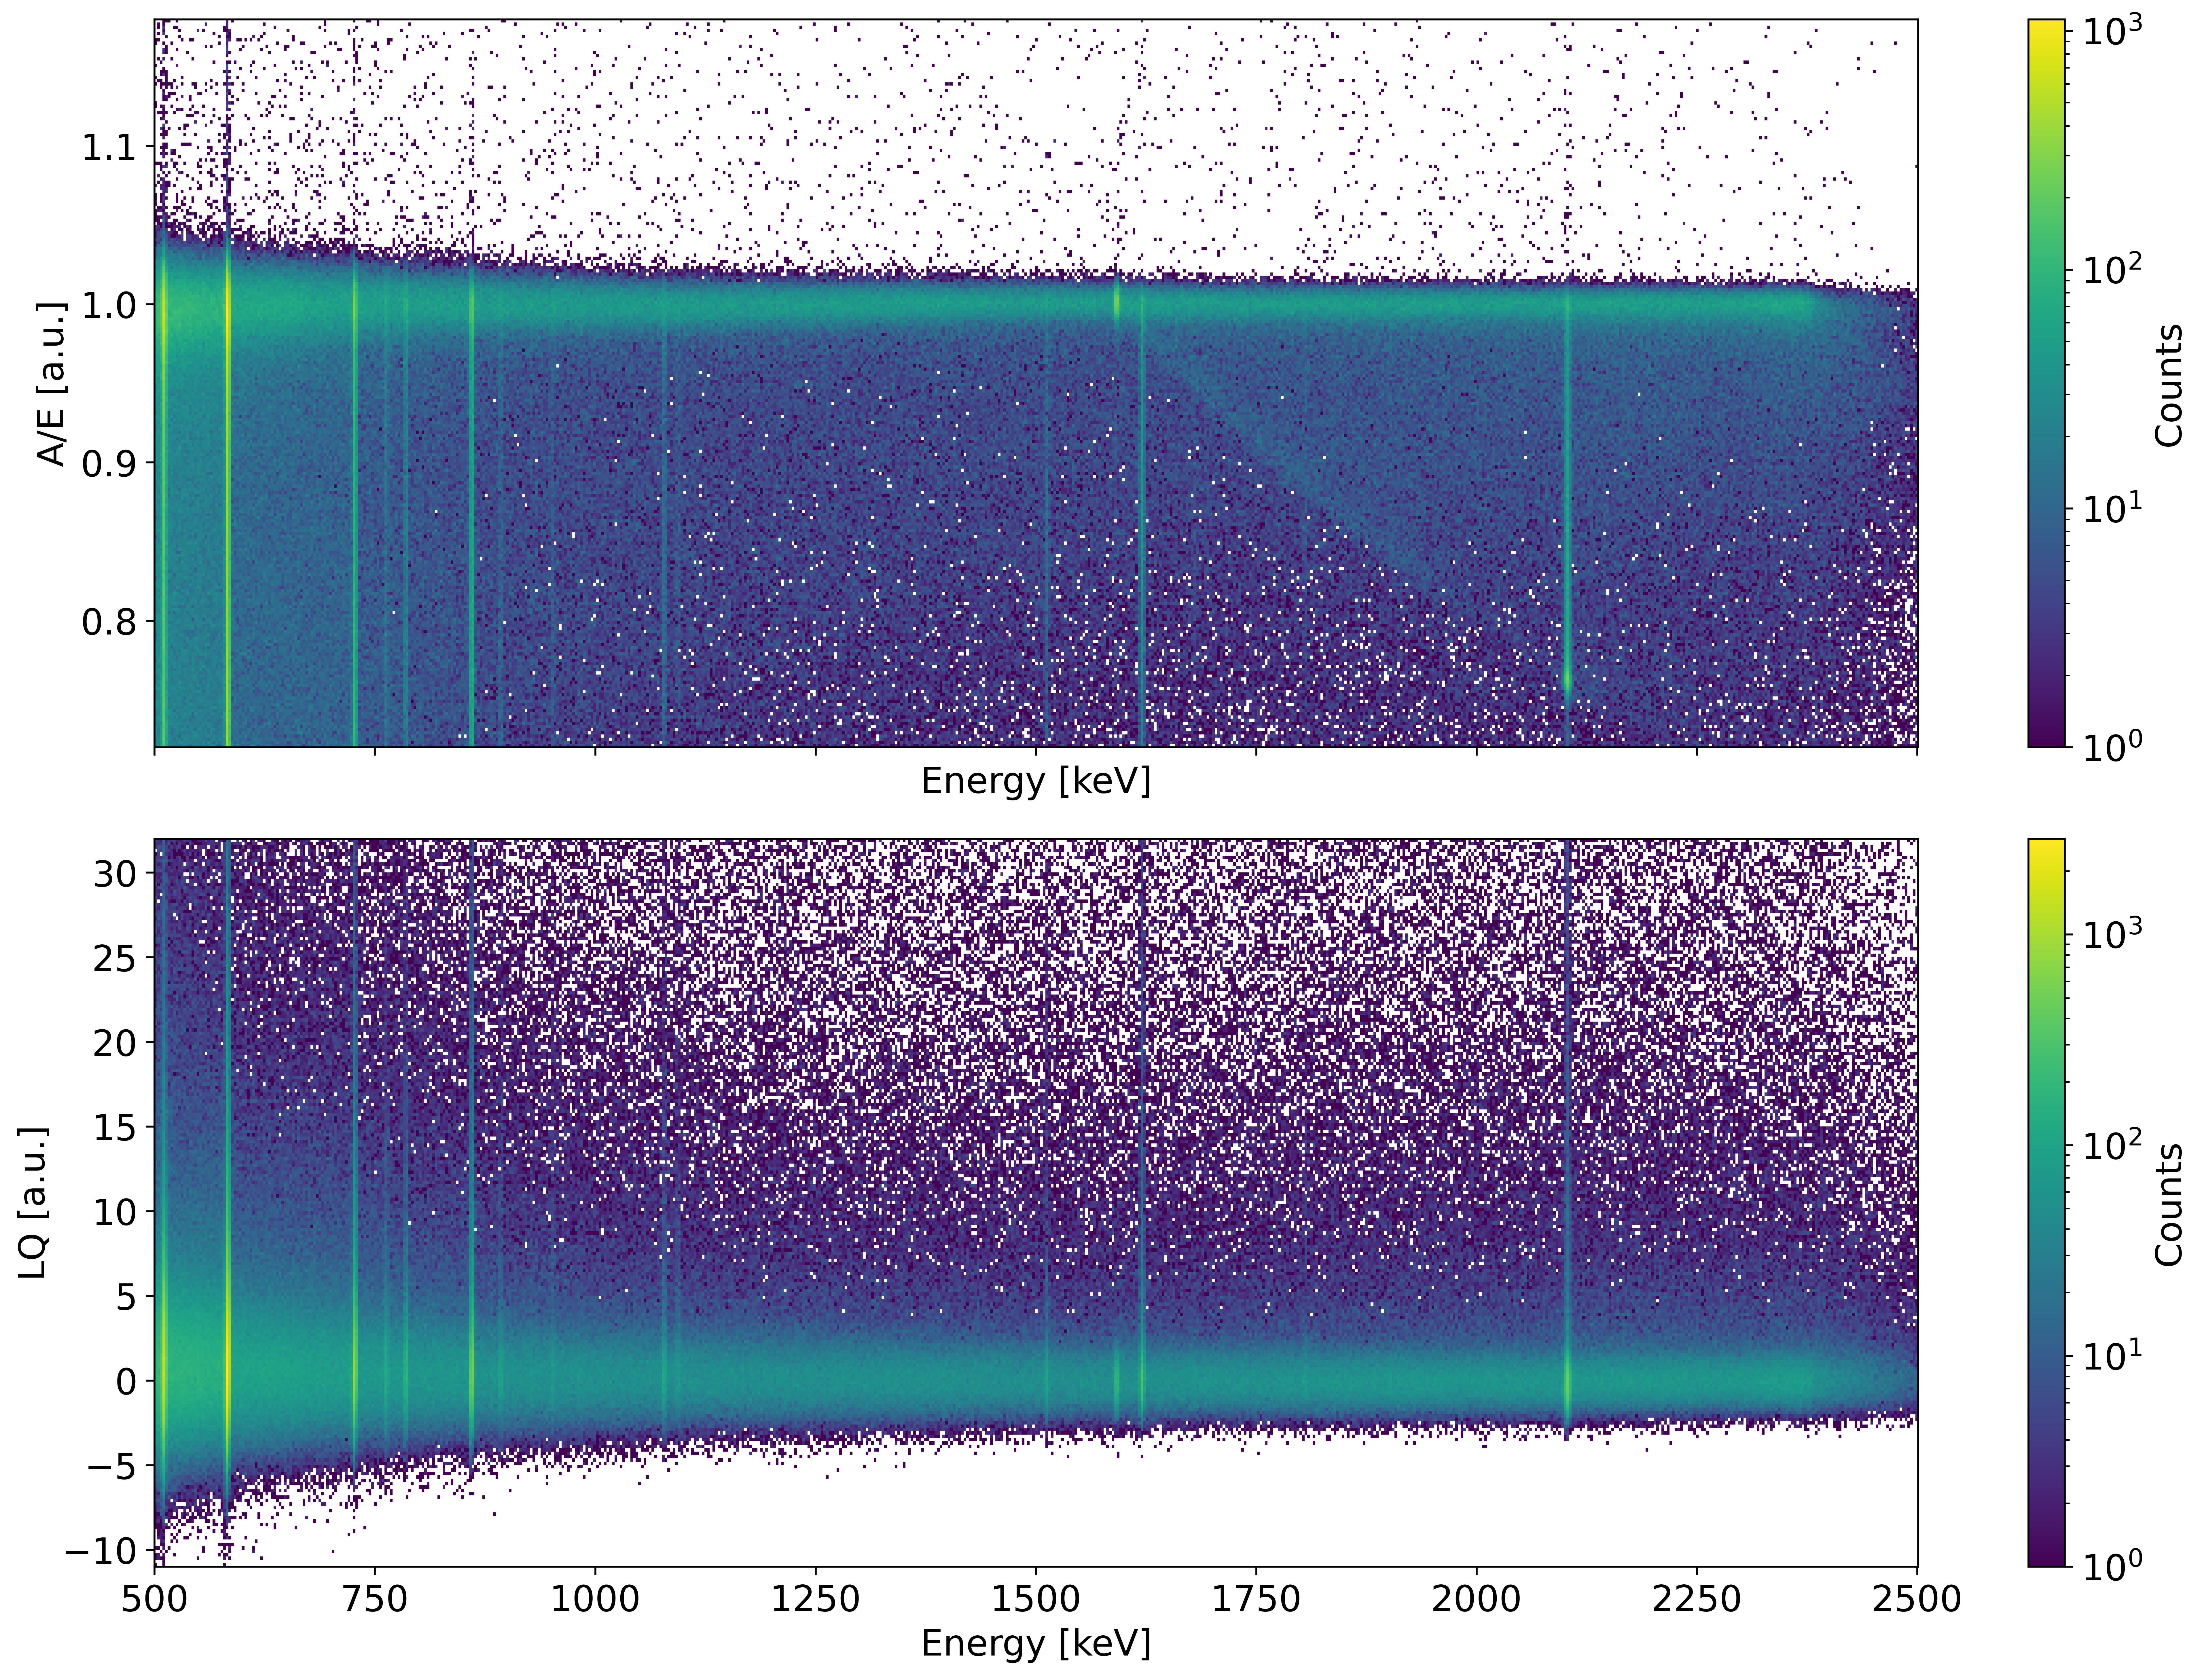
\includegraphics[width=0.85\linewidth]{figures/03_legend/Plot_Aoe_LQ_V09372A.png}
    \caption{Distributions of A/E (top) and LQ (bottom) as a function of energy for the same dataset as in figure~\ref{fig:Calibration_spectrum_Th228} ($^{228}$Th, period 9, run 3, detector V09372A). Both PSD parameters show a narrow single-site band, centered around 1 for A/E and around 0 for LQ, which is successfully corrected for energy dependence. }
    \label{fig:Aoe_LQ_spectra}
\end{figure}